\documentclass[a4paper]{article}

\def\npart {IB}
\def\nterm {Lent}
\def\nyear {2015}
\def\nlecturer {D.\ Tong}
\def\ncourse {Electromagnetism}
\def\nofficial {http://www.damtp.cam.ac.uk/user/tong/justem.html}

\usepackage{myheader}

\begin{document}
\maketitle
{\small
\noindent\textbf{Electromagnetism and Relativity}\\
Review of Special Relativity; tensors and index notation. Lorentz force law. Electromagnetic tensor. Lorentz transformations of electric and magnetic fields. Currents and the conservation of charge. Maxwell equations in relativistic and non-relativistic forms.\hspace*{\fill} [5]

\vspace{10pt}
\noindent\textbf{Electrostatics}\\
Gauss's law. Application to spherically symmetric and cylindrically symmetric charge distributions. Point, line and surface charges. Electrostatic potentials; general charge distributions, dipoles. Electrostatic energy. Conductors.\hspace*{\fill} [3]

\vspace{10pt}
\noindent\textbf{Magnetostatics}\\
Magnetic fields due to steady currents. Ampre's law. Simple examples. Vector potentials and the Biot-Savart law for general current distributions. Magnetic dipoles. Lorentz force on current distributions and force between current-carrying wires. Ohm's law.\hspace*{\fill} [3]

\vspace{10pt}
\noindent\textbf{Electrodynamics}\\
Faraday's law of induction for fixed and moving circuits. Electromagnetic energy and Poynting vector. 4-vector potential, gauge transformations. Plane electromagnetic waves in vacuum, polarization.\hspace*{\fill} [5]}

\tableofcontents

\setcounter{section}{-1}
\section{Introduction}
Electromagnetism is one of the four fundamental forces of the universe. Apart from gravity, most daily phenomena can be explained by electromagnetism. The very existence of atoms requires the electric force (plus weird quantum effects) to hold electrons to the nucleus, and molecules are formed again due to electric forces between atoms. More macroscopically, electricity powers all our electrical appliances (by definition), while the magnetic force makes things stick on our fridge. Finally, it is the force that gives rise to \emph{light}, and allows us to see things.

While it seems to be responsible for so many effects, the modern classical description of electromagnetism is rather simple. It is captured by merely \emph{four} short and concise equations known as Maxwell's equations. In fact, in the majority of this course, we would simply be exploring different solutions to these equations.

Historically, electromagnetism has another significance --- it led to Einstein's discovery of special relativity. At the end of the course, we will look at how Maxwell's equations naturally fit in nicely in the framework of relativity. Written relativistically, Maxwell's equation look \emph{much} simpler and more elegant. We will discover that magnetism is \emph{entirely} a relativistic effect, and makes sense only in the context of relativity.

As we move to the world of special relativity, not only do we get a better understanding of Maxwell's equation. As a takeaway, we also get to understand relativity itself better, as we provide a more formal treatment of special relativity, which becomes a powerful tool to develop theories consistent with relativity.

\section{Preliminaries}
\subsection{Charge and Current}
The strength of the electromagnetic force experienced by a particle is determined by its \emph{(electric) charge}. The SI unit of charge is the \emph{Coulomb}. In this course, we assume that the charge can be any real number. However, at the fundamental level, charge is quantised. All particles carry charge $q = ne$ for some integer $n$, and the basic unit $e \approx \SI{1.6e-19}{\coulomb}$. For example, the electron has $n = -1$, proton has $n = +1$, neutron has $n = 0$.

Often, it will be more useful to talk about \emph{charge density} $\rho(\mathbf{x}, t)$.
\begin{defi}[Charge density]
  The \emph{charge density} is the charge per unit volume. The total charge in a region $V$ is
  \[
    Q = \int_V \rho(\mathbf{x}, t)\; \d V
  \]
\end{defi}
When we study charged sheets or lines, the charge density would be charge per unit area or length instead, but this would be clear from context.

The motion of charge is described by the \emph{current} density $\mathbf{J}(\mathbf{x}, t)$.
\begin{defi}[Current and current density]
For any surface $S$, the integral
\[
  I = \int_S \mathbf{J}\cdot d\mathbf{S}
\]
counts the charge per unit time passing through $S$. $I$ is the \emph{current}, and $\mathbf{J}$ is the \emph{current density}, ``current per unit area''.
\end{defi}
Intuitively, if the charge distribution $\rho (\mathbf{x}, t)$ has velocity $\mathbf{v}(x, t)$, then (neglecting relativistic effects), we have
\[
  \mathbf{J} = \rho \mathbf{v}.
\]

\begin{eg}
  A wire is a cylinder of cross-sectional area $A$. Suppose there are $n$ electrons per unit volume. Then
  \begin{align*}
    \rho &= nq = -ne\\
    \mathbf{J} &= nq\mathbf{v}\\
    I &= nqvA.
  \end{align*}
\end{eg}

It is well known that charge is conserved --- we cannot create or destroy charge. However, the conservation of charge does not simply say that ``the total charge in the universe does not change''. We want to rule out scenarios where a charge on Earth disappears, and instantaneously appears on the Moon. So what we really want to say is that charge is conserved locally: if it disappears here, it must have moved to somewhere nearby. Alternatively, charge density can only change due to continuous currents. This is captured by the \emph{continuity equation}:
\begin{law}[Continuity equation]
  \[
    \frac{\partial\rho}{\partial t} + \nabla\cdot \mathbf{J} = 0.
  \]
\end{law}
We can write this into a more intuitive integral form via the divergence theorem.

The charge $Q$ in some region $V$ is defined to be
\[
  Q = \int_V \rho \;\d V.
\]
So
\[
  \frac{\d Q}{\d t} = \int_V \frac{\partial\rho}{\partial t}\; \d V = -\int_V \nabla\cdot \mathbf{J}\; \d V = -\int_S \mathbf{J}\cdot \d S.
\]
Hence the continuity equation states that the change in total charge in a volume is given by the total current passing through its boundary.

In particular, we can take $V = \R^3$, the whole of space. If there are no currents at infinity, then
\[
  \frac{\d Q}{\d t} = 0
\]
So the continuity equation implies the conservation of charge.

\subsection{Forces and Fields}
In modern physics, we believe that all forces are mediated by \emph{fields} (not to be confused with ``fields'' in algebra, or agriculture). A \emph{field} is a dynamical quantity (i.e.\ a function) that assigns a value to every point in space and time. In electromagnetism, we have two fields:
\begin{itemize}
  \item the electric field $\mathbf{E}(\mathbf{x}, t)$;
  \item the magnetic field $\mathbf{B}(\mathbf{x}, t)$.
\end{itemize}
Each of these fields is a vector, i.e.\ it assigns a \emph{vector} to every point in space and time, instead of a single number.

The fields interact with particles in two ways. On the one hand, fields cause particles to move. On the other hand, particles create fields. The first aspect is governed by the Lorentz force law:
\begin{law}[Lorentz force law]
\[
  \mathbf{F} = q(\mathbf{E} + \mathbf{v}\times \mathbf{B})
\]
\end{law}
\noindent while the second aspect is governed by \emph{Maxwell's equations}.
\begin{law}[Maxwell's Equations]
  \begin{align*}
    \nabla \cdot \mathbf{E} &= \frac{\rho}{\varepsilon_0}\\
    \nabla \cdot \mathbf{B} &= 0\\
    \nabla \times \mathbf{E} +\frac{\partial \mathbf{B}}{\partial t} &= 0\\
    \nabla \times \mathbf{B} - \mu_0\varepsilon_0 \frac{\partial \mathbf{E}}{\partial t} &= \mu_0 \mathbf{J},
  \end{align*}
  where we have two constants of nature:
  \begin{itemize}
    \item $\varepsilon_0 = \SI{8.85e-12}{\per\metre\cubed\per\kilogram\s\squared\coulomb\squared}$ is the electric constant;
    \item $\mu_0 = \SI{4\pi e-6}{\metre\kilogram\per\coulomb\squared}$ is the magnetic constant.
  \end{itemize}
  Some prefer to call these constants the ``permittivity of free space'' and ``permeability of free space'' instead. But why bother with these complicated and easily-confused names when we can just call them ``electric constant'' and ``magnetic constant''?
\end{law}
We've just completed the description of all of (classical, non-relativistic) electromagnetism. The remaining of the course would be to study the consequences of and solutions to these equations.

\section{Electrostatics}
Electrostatics is the study of stationary charges in the absence of magnetic fields. We take $\rho = \rho(\mathbf{x})$, $\mathbf{J} = 0$ and $\mathbf{B} = 0$. We then look for time-independent solutions. In this case, the only relevant equations are
\begin{align*}
  \nabla \cdot \mathbf{E} &= \frac{\rho}{\varepsilon_0}\\
  \nabla\times \mathbf{E} &= 0,
\end{align*}
and the other two equations just give $0 = 0$.

In this chapter, our goal is to find $\mathbf{E}$ for any $\rho$. Of course, we first start with simple, symmetric cases, and then tackle the more general cases later.

\subsection{Gauss' Law}
Here we transform the first Maxwell's equation into an integral form, known as \emph{Gauss' Law}.

Consider a region $V\subseteq \R^3$ with boundary $S = \partial V$. Then integrating the first equation over the volume $V$ gives
\[
  \int_V \nabla\cdot \mathbf{E}\; \d V = \frac{1}{\varepsilon_0} \int_V \rho \;\d V.
\]
The divergence theorem gives $\int_V \nabla\cdot \mathbf{E}\;\d V = \int_S \mathbf{E}\cdot \d \mathbf{S}$, and by definition, $Q = \int_V \rho \;\d V$. So we end up with
\begin{law}[Gauss' law]
  \[
    \int_S \mathbf{E}\cdot \d \mathbf{S} =\frac{Q}{\varepsilon_0},
  \]
  where $Q$ is the total charge inside $V$.
\end{law}
\begin{defi}[Flux through surface]
  The \emph{flux} of $\mathbf{E}$ through the surface $S$ is defined to be
  \[
    \int_S \mathbf{E} \cdot\d \mathbf{S}.
  \]
\end{defi}

Gauss' law tells us that the flux depends only on the total charge contained inside the surface. In particular any external charge does not contribute to the total flux. While external charges \emph{do} create fields that pass through the surface, the fields have to enter the volume through one side of the surface and leave through the other. Gauss' law tells us that these two cancel each other out exactly, and the total flux caused by external charges is zero.

From this, we can prove Coulomb's law:
\begin{eg}[Coulomb's law]
  We consider a spherically symmetric charge density $\rho (r)$ with $\rho (r) = 0$ for $r > R$, i.e.\ all the charge is contained in a ball of radius $R$.
  \begin{center}
    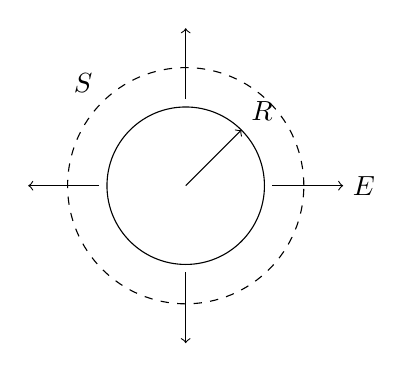
\begin{tikzpicture}
      \draw circle [radius=1];
      \draw [->] (0, 0) -- (.71, .71) node [anchor=south west] {$R$};
      \draw [->] (0, 1.1) -- (0, 2);
      \draw [->] (0, -1.1) -- (0, -2);
      \draw [->] (1.1, 0) -- (2, 0) node [right] {$E$};
      \draw [->] (-1.1, 0) -- (-2, 0);
      \draw [dashed] circle [radius=1.5];
      \node at (-1.06, 1.06) [anchor=south east] {$S$};
    \end{tikzpicture}
  \end{center}
  By symmetry, the force is the same in all directions and point outward radially. So
  \[
    \mathbf{E} = E(r) \hat{\mathbf{r}}.
  \]
  This immediately ensures that $\nabla \times \mathbf{E} = 0$.

  Put $S$ to be a sphere of radius $r > R$. Then the total flux is
  \begin{align*}
    \int_S \mathbf{E}\cdot \d \mathbf{S} &= \int_S E(r) \hat{\mathbf{r}}\cdot \d \mathbf{S}\\
    &= E(r) \int_S \hat{\mathbf{r}}\cdot \d \mathbf{S}\\
    &= E(r)\cdot 4\pi r^2
  \end{align*}
  By Gauss' law, we know that this is equal to $\frac{Q}{\varepsilon_0}$. Therefore
  \[
    E(r) = \frac{Q}{4\pi \varepsilon_0 r^2}
  \]
  and
  \[
    \mathbf{E}(r) = \frac{Q}{4\pi\varepsilon_0 r^2}\hat{\mathbf{r}}.
  \]
  By the Lorentz force law, the force experienced by a second charge is
  \[
    \mathbf{F}(\mathbf{r}) = \frac{Qq}{4\pi\varepsilon_0 r^2}\hat{\mathbf{r}},
  \]
  which is Coulomb's law.

  Strictly speaking, this only holds when the charges are not moving. However, for most practical purposes, we can still use this because the corrections required when they are moving are tiny.
\end{eg}

\begin{eg}
  Consider a uniform sphere with
  \[
    \rho (r) = \begin{cases}
      \rho & r < R\\
      0 & r > R
    \end{cases}.
  \]
  Outside, we know that
  \[
    \mathbf{E}(r) = \frac{Q}{4\pi\varepsilon_0 r^2}\hat{\mathbf{r}}
  \]
  Now suppose we are inside the sphere.
  \begin{center}
    \begin{tikzpicture}
      \draw circle [radius=1];
      \draw [->] (0, 0) -- (.71, .71) node [anchor=south west] {$R$};
      \draw [->] (0, 1.1) -- (0, 2);
      \draw [->] (0, -1.1) -- (0, -2);
      \draw [->] (1.1, 0) -- (2, 0) node [right] {$E$};
      \draw [->] (-1.1, 0) -- (-2, 0);
      \draw [dashed] circle [radius=0.5];
      \draw [->] (0, 0) -- (-.353, .353) node [anchor=south east] {$r$};
    \end{tikzpicture}
  \end{center}
  Then
  \[
    \int_S \mathbf{E}\cdot \d\mathbf{S} = E(r) 4\pi r^2 = \frac{Q}{\varepsilon_0}\left(\frac{r^3}{R^3}\right)
  \]
  So
  \[
    \mathbf{E}(r) = \frac{Qr}{4\pi\varepsilon_0 R^3}\hat{\mathbf{r}},
  \]
  and the field increases with radius.
\end{eg}

\begin{eg}[Line charge]
  Consider an infinite line with uniform charge density \emph{per unit length} $\eta$.

  We use cylindrical polar coordinates:
  \begin{center}
    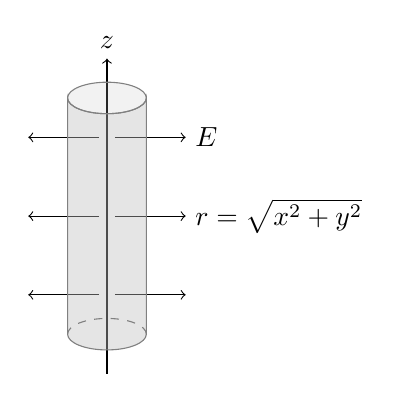
\begin{tikzpicture}
      \draw [->] (0, -2) -- (0, 2) node [above] {$z$};
      \draw [->] (0.1, 0) -- (1, 0) node [right] {$r = \sqrt{x^2 + y^2}$};

      \draw [->] (0.1, 1) -- (1, 1) node [right] {$E$};
      \draw [->] (-0.1, 1) -- (-1, 1);
      \draw [->] (-0.1, 0) -- (-1, 0);
      \draw [->] (0.1, -1) -- (1, -1);
      \draw [->] (-0.1, -1) -- (-1, -1);

      \draw [gray, fill=gray!50!white, fill opacity=0.4] (-0.5, 1.5) arc (180:360:0.5 and 0.2) -- (0.5, -1.5) arc (360:180:0.5 and 0.2) -- cycle;
      \draw [gray, fill=gray!50!white, fill opacity=0.2] (0, 1.5) circle [x radius=0.5, y radius=0.2];
      \draw [gray, dashed] (0.5, -1.5) arc (0:180:0.5 and 0.2);
    \end{tikzpicture}
  \end{center}
  By symmetry, the field is radial, i.e.
  \[
    \mathbf{E}(r) = E(r) \hat{\mathbf{r}}.
  \]
  Pick $S$ to be a cylinder of length $L$ and radius $r$. We know that the end caps do not contribute to the flux since the field lines are perpendicular to the normal. Also, the curved surface has area $2\pi rL$. Then
  \[
    \int_S\mathbf{E}\cdot \d\mathbf{S} = E(r)2\pi rL = \frac{\eta L}{\varepsilon_0}.
  \]
  So
  \[
    \mathbf{E}(r) = \frac{\eta}{2\pi \varepsilon_0 r} \hat{\mathbf{r}}.
  \]
  Note that the field varies as $1/r$, not $1/r^2$. Intuitively, this is because we have one more dimension of ``stuff'' compared to the point charge, so the field does not drop as fast.
\end{eg}

\begin{eg}[Surface charge]
  Consider an infinite plane $z = 0$, with uniform charge per unit area $\sigma$.
  \begin{center}
    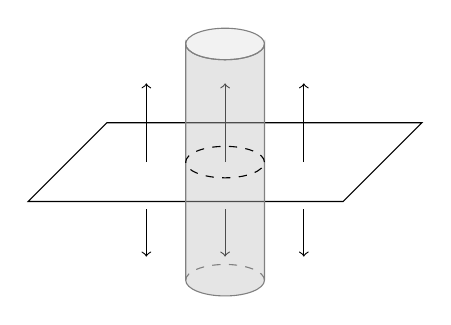
\begin{tikzpicture}
      \draw (-2.5, -.5) -- (1.5, -.5) -- (2.5, .5) -- (-1.5, .5) -- cycle;
      \draw [->] (0, 0) -- (0, 1);
      \draw [->] (-1, 0) -- (-1, 1);
      \draw [->] (1, 0) -- (1, 1);

      \draw [->] (0, -.6) -- (0, -1.2);
      \draw [->] (1, -.6) -- (1, -1.2);
      \draw [->] (-1, -.6) -- (-1, -1.2);

      \draw [gray, fill=gray!50!white, fill opacity=0.4] (-0.5, 1.5) arc (180:360:0.5 and 0.2) -- (0.5, -1.5) arc (360:180:0.5 and 0.2) -- cycle;
      \draw [gray, fill=gray!50!white, fill opacity=0.2] (0, 1.5) circle [x radius=0.5, y radius=0.2];
      \draw [gray, dashed] (0.5, -1.5) arc (0:180:0.5 and 0.2);

      \draw [dashed] circle [x radius=0.5, y radius=0.2];
    \end{tikzpicture}
  \end{center}
  By symmetry, the field points vertically, and the field bottom is the opposite of that on top. we must have
  \[
    \mathbf{E} = E(z)\hat{\mathbf{z}}
  \]
  with
  \[
    E(z) = -E(-z).
  \]
  Consider a vertical cylinder of height $2z$ and cross-sectional area $A$. Now only the end caps contribute. So
  \[
    \int_S \mathbf{E} \cdot \d \mathbf{S} = E(z) A - E(-z) A =\frac{\sigma A}{\varepsilon _0}.
  \]
  So
  \[
    E(z) = \frac{\sigma }{2\varepsilon_0}
  \]
  and is constant.

  Note that the electric field is discontinuous across the surface. We have
  \[
    E(z\to 0+) - E(z\to 0-) = \frac{\sigma}{\varepsilon_0}.
  \]
  This is a general result that is true for any arbitrary surfaces and $\sigma$. We can prove this by considering a cylinder across the surface and then shrink it indefinitely. Then we find that
  \[
    \hat{\mathbf{n}}\cdot \mathbf{E}_+ - \hat{\mathbf{n}}\cdot \mathbf{E}_- = \frac{\sigma}{\varepsilon_0}.
  \]
  However, the components of $\mathbf{E}$ tangential to the surface are continuous.
\end{eg}

\subsection{Electrostatic potential}
In the most general case, we will have to solve both $\nabla \cdot \mathbf{E} = \rho/\varepsilon_0$ and $\nabla \times \mathbf{E} = \mathbf{0}$. However, we already know that the general form of the solution to the second equation is $\mathbf{E} = -\nabla\phi$ for some scalar field $\phi$.
\begin{defi}[Electrostatic potential]
  If $\mathbf{E} = -\nabla \phi$, then $\phi$ is the \emph{electrostatic potential}.
\end{defi}
Substituting this into the first equation, we obtain
\[
  \nabla^2\phi = \frac{\rho}{\varepsilon_0}.
\]
This is the \emph{Poisson equation}, which we have studied in other courses. If we are in the middle of nowhere and $\rho = 0$, then we get the \emph{Laplace equation}.

There are a few interesting things to note about our result:
\begin{itemize}
  \item $\phi$ is only defined up to a constant. We usually fix this by insisting $\phi(\mathbf{r}) \to 0$ as $r\to \infty$. This statement seems trivial, but this property of $\phi$ is actually very important and gives rise to a lot of interesting properties. However, we will not have the opportunity to explore this in this course.
  \item The Poisson equation is linear. So if we have two charges $\rho_1$ and $\rho_2$, then the potential is simply $\phi_1 + \phi_2$ and the field is $\mathbf{E}_1 + \mathbf{E}_2$. This is the \emph{principle of superposition}. Among the four fundamental forces of nature, electromagnetism is the only force with this property.
\end{itemize}
\subsubsection{Point charge}
Consider a point particle with charge $Q$ at the origin. Then
\[
  \rho (\mathbf{r}) = Q\delta^3(\mathbf{r}).
\]
Here $\delta^3$ is the generalization of the usual delta function for (3D) vectors.

The equation we have to solve is
\[
  \nabla^2\phi = -\frac{Q}{\varepsilon_0}\delta^3(\mathbf{r}).
\]
Away from the origin $\mathbf{r} = \mathbf{0}$, $\delta^3(\mathbf{r}) = 0$, and we have the Laplace equation. From the IA Vector Calculus course, the general solution is
\[
  \phi = \frac{\alpha}{r}\quad \text{for some constant }\alpha.
\]
The constant $\alpha$ is determined by the delta function. We integrate the equation over a sphere of radius $r$ centered at the origin. The left hand side gives
\[
  \int_V \nabla^2\phi\;\d V = \int_S \nabla\phi\cdot\d \mathbf{S} = \int_S -\frac{\alpha}{r^2} \hat{\mathbf{r}}\cdot \d \mathbf{S} = -4\pi\alpha
\]
The right hand side gives
\[
  -\frac{Q}{\varepsilon_0}\int_V\delta^3(r)\; \d V = -\frac{Q}{\varepsilon_0}.
\]
So
\[
  \alpha = \frac{Q}{4\pi \varepsilon_0}
\]
and
\[
  \mathbf{E} = -\nabla \phi = \frac{Q}{4\pi\varepsilon_0 r^2}\hat{\mathbf{r}}.
\]
This is just what we get from Coulomb's law.
\subsubsection{Dipole}
\begin{defi}[Dipole]
  A \emph{dipole} consists of two point charges, $+Q$ and $-Q$ at $\mathbf{r} = 0$ and $\mathbf{r} = -\mathbf{d}$ respectively.
\end{defi}

To find the potential of a dipole, we simply apply the principle of superposition and obtain
\[
  \phi = \frac{1}{4\pi\varepsilon_0}\left(\frac{Q}{r} - \frac{Q}{|\mathbf{r} + \mathbf{d}|}\right).
\]
This is not a very helpful result, but we can consider the case when we are far, far away, i.e.\ $r \gg d$. To do so, we Taylor expand the second term. For a general $f(\mathbf{r})$, we have
\[
  f(\mathbf{r} + \mathbf{d}) = f(\mathbf{r}) + \mathbf{d}\cdot \nabla f(\mathbf{r}) + \frac{1}{2}(\mathbf{d}\cdot \nabla)^2f(\mathbf{r}) + \cdots.
\]
Applying to the term we are interested in gives
\begin{align*}
  \frac{1}{|\mathbf{r} + \mathbf{d}|} &= \frac{1}{r} - \mathbf{d}\cdot \nabla\left(\frac{1}{r}\right) + \frac{1}{2}(\mathbf{d}\cdot \nabla)^2\left(\frac{1}{r}\right) + \cdots\\
  &= \frac{1}{r} - \frac{\mathbf{d}\cdot \mathbf{r}}{r^3} - \frac{1}{2}\left(\frac{\mathbf{d}\cdot \mathbf{d}}{r^3} - \frac{3(\mathbf{d}\cdot \mathbf{r})^2}{r^5}\right) + \cdots.
\end{align*}
Plugging this into our equation gives
\[
  \phi = \frac{Q}{4\pi\varepsilon_0}\left(\frac{1}{r} - \frac{1}{r} + \frac{\mathbf{d}\cdot \mathbf{r}}{r^3} + \cdots\right) \sim \frac{Q}{4\pi\varepsilon_0} \frac{\mathbf{d}\cdot \mathbf{r}}{r^3}.
\]
\begin{defi}[Electric dipole moment]
  We define the \emph{electric dipole moment} to be
  \[
    \mathbf{p} = Q\mathbf{d}.
  \]
  By convention, it points from -ve to +ve.
\end{defi}
Then
\[
  \phi = \frac{\mathbf{p}\cdot \hat{\mathbf{r}}}{4\pi\varepsilon_0 r^2},
\]
and
\[
  \mathbf{E} = -\nabla\phi = \frac{1}{4\pi\varepsilon_0}\left(\frac{3(\mathbf{p}\cdot\hat{\mathbf{r}})\hat{\mathbf{r}} - \mathbf{p}}{r^3}\right).
\]

\subsubsection{General charge distribution}
To find $\phi$ for a general charge distribution $\rho$, we use the Green's function for the Laplacian. The Green's function is defined to be the solution to
\[
  \nabla^2 G(\mathbf{r}, \mathbf{r}') = \delta^3(\mathbf{r} - \mathbf{r}'),
\]
In the section about point charges, We have shown that
\[
  G(\mathbf{r}, \mathbf{r}') = -\frac{1}{4\pi}\frac{1}{|\mathbf{r} - \mathbf{r}'|}.
\]
We assume all charge is contained in some compact region $V$. Then
\begin{align*}
  \phi(\mathbf{r}) &= -\frac{1}{\varepsilon_0}\int_V \rho(\mathbf{r}') G(\mathbf{r}, \mathbf{r}')\;\d^3 \mathbf{r}'\\
  &= \frac{1}{4\pi\varepsilon_0}\int_V \frac{\rho(\mathbf{r}')}{|\mathbf{r} - \mathbf{r}'|}\;\d^3 \mathbf{r}'
\end{align*}
Then
\begin{align*}
  \mathbf{E}(\mathbf{r}) &= -\nabla \phi(\mathbf{r})\\
  &=- \frac{1}{4\pi\varepsilon_0} \int_V \rho(\mathbf{r}')\nabla \left(\frac{1}{|\mathbf{r} - \mathbf{r}'|}\right)\;\d^3 \mathbf{r}'\\
  &= \frac{1}{4\pi\varepsilon_0}\int_V \rho(\mathbf{r}')\frac{(\mathbf{r} - \mathbf{r}')}{|\mathbf{r} - \mathbf{r}'|^3}\;\d^3 \mathbf{r}'
\end{align*}
So if we plug in a very complicated $\rho$, we get a very complicated $\mathbf{E}$!

However, we can ask what $\phi$ and $\mathbf{E}$ look like very far from $V$, i.e.\ $|\mathbf{r}| \gg |\mathbf{r}'|$.

We again use the Taylor expansion.
\begin{align*}
  \frac{1}{|\mathbf{r} - \mathbf{r}'|} &= \frac{1}{r} + \mathbf{r}'\cdot \nabla\left(\frac{1}{r}\right) + \cdots\\
  &= \frac{1}{r} + \frac{\mathbf{r}\cdot \mathbf{r}'}{r^3} + \cdots.
\end{align*}
Then we get
\begin{align*}
  \phi(\mathbf{r}) &= \frac{1}{4\pi\varepsilon_0} \int_V \rho(\mathbf{r}')\left(\frac{1}{r} + \frac{\mathbf{r}\cdot \mathbf{r}'}{r^3} + \cdots\right)\;\d^3 \mathbf{r}'\\
  &= \frac{1}{4\pi\varepsilon_0}\left(\frac{Q}{r} + \frac{\mathbf{p}\cdot \hat{\mathbf{r}}}{r^2} + \cdots\right),
\end{align*}
where
\begin{align*}
  Q &= \int_V \rho(\mathbf{r}')\;\d V' \\
  \mathbf{p} &= \int_V \mathbf{r}'\rho(\mathbf{r}')\; \d V'\\
  \hat{\mathbf{r}} &= \frac{\mathbf{r}}{\|\mathbf{r}\|}.
\end{align*}
So if we have a huge lump of charge, we can consider it to be a point charge $Q$, plus some dipole correction terms.
\subsubsection{Field lines and equipotentials}
Vectors are usually visualized using arrows, where longer arrows represent larger vectors. However, this is not a practical approach when it comes to visualizing fields, since a field assigns a vector to \emph{every single point in space}, and we don't want to draw infinitely many arrows. Instead, we use field lines.

\begin{defi}[Field line]
  A \emph{field line} is a continuous line tangent to the electric field $\mathbf{E}$. The density of lines is proportional to $|\mathbf{E}|$.
\end{defi}
They begin and end only at charges (and infinity), and never cross.

We can also draw the \emph{equipotentials}.
\begin{defi}[Equipotentials]
  \emph{Equipotentials} are surfaces of constant $\phi$. Because $\mathbf{E} = -\nabla \phi$, they are always perpendicular to field lines.
\end{defi}
\begin{eg}\leavevmode
  The field lines for a positive and a negative charge are, respectively,
  \begin{center}
    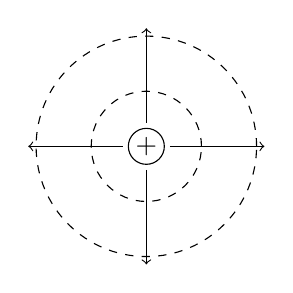
\begin{tikzpicture}
      \node [draw, circle, inner sep = 0, minimum size=13] {+};
      \draw [dashed] circle [radius=1.4];
      \draw [dashed] circle [radius=.7];
      \draw [->] (0, 0.3) -- (0, 1.5);
      \draw [->] (0.3, 0) -- (1.5, 0);
      \draw [->] (0, -0.3) -- (0, -1.5);
      \draw [->] (-0.3, 0) -- (-1.5, 0);
    \end{tikzpicture}
    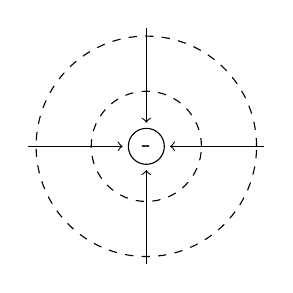
\begin{tikzpicture}
      \node [draw, circle, inner sep = 0, minimum size=13] {-};
      \draw [dashed] circle [radius=1.4];
      \draw [dashed] circle [radius=.7];
      \draw [->] (0, 1.5) -- (0, 0.3);
      \draw [->] (1.5, 0) -- (0.3, 0);
      \draw [->] (0, -1.5) -- (0, -0.3);
      \draw [->] (-1.5, 0) -- (-0.3, 0);
    \end{tikzpicture}
  \end{center}
  We can also draw field lines for dipoles:
  \begin{center}
    \begin{tikzpicture}
      \node [draw, circle, inner sep = 0, minimum size=13] (+) {+};
      \node [draw, circle, inner sep = 0, minimum size=13] (-) at (2, 0) {-};
      \draw [->-=0.6] (+) -- (-);
      \draw [->-=0.6] (+) to [bend left=30] (-);
      \draw [->-=0.6] (+) to [bend right=30] (-);
      \draw [->-=0.6] (+) to [bend left=60] (-);
      \draw [->-=0.6] (+) to [bend right=60] (-);
      \draw [->-=0.7] (+) to [bend right=30] +(-1, 0.5);
      \draw [->-=0.7] (+) to [bend left=30] +(-1, -0.5);
      \draw [->-=0.7] (+) to +(-1, 0);
      \draw [-<-=0.4] (-) to [bend left=30] +(1, 0.5);
      \draw [-<-=0.4] (-) to [bend right=30] +(1, -0.5);
      \draw [-<-=0.4] (-) to +(1, 0);
    \end{tikzpicture}
  \end{center}
\end{eg}

\subsection{Electrostatic energy}
We want to calculate how much energy is stored in the electric field. Recall from IA Dynamics and Relativity that a particle of charge $q$ in a field $\mathbf{E} = -\nabla \phi$ has potential energy $U(\mathbf{r}) = q\phi(\mathbf{r})$.

$U(\mathbf{r})$ can be thought of as the work done in bringing the particle from infinity, as illustrated below:
\begin{align*}
  \text{work done} &= -\int_\infty^\mathbf{r} \mathbf{F}\cdot \d \mathbf{r}\\
  &= -\int_\infty^\mathbf{r}\mathbf{E}\cdot \d \mathbf{r} \\
  &= q\int_\infty^\mathbf{r} \nabla \mathbf{\phi}\cdot \d \mathbf{r}\\
  &= q[\phi(\mathbf{r}) - \phi(\infty)]\\
  &= U(\mathbf{r})
\end{align*}
where we set $\phi(\infty) = 0$.

Now consider $N$ charges $q_i$ at positions $\mathbf{r}_i$. The total potential energy stored is the work done to assemble these particles. Let's put them in one by one.
\begin{enumerate}
  \item The first charge is free. The work done is $W_1 = 0$.
  \item To place the second charge at position $\mathbf{r}_2$ takes work. The work is
    \[
      W_2 = \frac{q_1q_2}{4\pi\varepsilon_0}\frac{1}{|\mathbf{r}_1 - \mathbf{r}_2|}.
    \]
  \item To place the third charge at position $\mathbf{r}_3$, we do
    \[
      W_3 = \frac{q_3}{4\pi\varepsilon_0}\left(\frac{q_1}{|\mathbf{r}_1 - \mathbf{r}_3|} + \frac{q_2}{|\mathbf{r}_2 - \mathbf{r}_3|}\right)
    \]
  \item etc.
\end{enumerate}
The total work done is
\[
  U = \sum_{i = 1}^N W_i = \frac{1}{4\pi\varepsilon_0} \sum_{i < j} \frac{q_iq_j}{|\mathbf{r}_i - \mathbf{r}_j|}.
\]
Equivalently,
\[
  U = \frac{1}{4\pi\varepsilon_0} \frac{1}{2} \sum_{i \not= j} \frac{q_iq_j}{|\mathbf{r}_i - \mathbf{r}_j|}.
\]
We can write this in an alternative form. The potential at point $\mathbf{r}_i$ due to all other particles is
\[
  \phi(\mathbf{r}_i) = \frac{1}{4\pi\varepsilon_0}\sum_{j\not= i}\frac{q_j}{|\mathbf{r}_i - \mathbf{r}_j|}.
\]
So we can write
\[
  U = \frac{1}{2}\sum_{i = 1}^N q_i \phi(\mathbf{r}_i).
\]
There is an obvious generalization to continuous charge distributions:
\[
  U = \frac{1}{2} \int \rho (\mathbf{r}) \phi(\mathbf{r}) \;\d^3 \mathbf{r}.
\]
Hence we obtain
\begin{align*}
  U &= \frac{\varepsilon_0}{2}\int (\nabla\cdot \mathbf{E}) \phi \;\d^3 \mathbf{r}\\
  &= \frac{\varepsilon_0}{2}\int [\nabla\cdot (\mathbf{E}\phi) - \mathbf{E}\cdot \nabla \phi]\;\d^3 \mathbf{r}.
\end{align*}
The first term is a total derivative and vanishes. In the second term, we use the definition $\mathbf{E} = -\nabla \phi$ and obtain
\begin{prop}
  \[
    U = \frac{\varepsilon_0}{2}\int \mathbf{E}\cdot \mathbf{E} \;\d^3 \mathbf{r}.
  \]
\end{prop}
This derivation of potential energy is not satisfactory. The final result shows that the potential energy depends only on the field itself, and not the charges. However, the result was derived using charges and electric potentials --- there should be a way to derive this result directly with the field, and indeed there is. However, this derivation belongs to a different course.

Also, we have waved our hands a lot when generalizing to continuous distributions, which was not entirely correct. If we have a single point particle, the original discrete formula implies that there is no potential energy. However, since the associated field is non-zero, our continuous formula gives a non-zero potential.

This does \emph{not} mean that the final result is wrong. It is correct, but it describes a more sophisticated (and preferred) conception of ``potential energy''. Again, we shall not go into the details in this course.

\subsection{Conductors}
\begin{defi}[Conductor]
  A \emph{conductor} is a region of space which contains lots of charges that are free to move.
\end{defi}

In electrostatic situations, we must have $\mathbf{E} = 0$ inside a conductor. Otherwise, the charges inside the conductor would move till equilibrium. This almost describes the whole of the section: if you apply an electric field onto a conductor, the charges inside the conductor move until the external field is canceled out.

From this, we can derive a lot of results. Since $\mathbf{E} = 0$, $\phi$ is constant inside the conductor. Since $\nabla \cdot \mathbf{E} = \rho/\varepsilon_0$, inside the conductor, we must have $\rho = 0$. Hence any net charge must live on the surface.

Also, since $\phi$ is constant inside the conductor, the surface of the conductor is an equipotential. Hence the electric field is perpendicular to the surface. This makes sense since any electric field with components parallel to the surface would cause the charges to move.

Recall also from our previous discussion that across a surface, we have
\[
  \hat{\mathbf{n}}\cdot \mathbf{E}_\text{outside} - \hat{\mathbf{n}}\cdot \mathbf{E}_\text{inside} = \frac{\sigma}{\varepsilon_0},
\]
where $\sigma$ is the surface charge density. Since $\mathbf{E}_\text{inside} = 0$, we obtain
\[
  \mathbf{E}_\text{outside} = \frac{\sigma}{\varepsilon_0}\hat{\mathbf{n}}
\]
This allows us to compute the surface charge given the field, and vice versa.

\begin{eg}
  Consider a spherical conductor with $Q = 0$. We put a positive plate on the left and a negative plate on the right. This creates a field from the left to the right.

  With the conductor in place, since the electric field lines must be perpendicular to the surface, they have to bend towards the conductor. Since field lines end and start at charges, there must be negative charges at the left and positive charges at the right.
  \begin{center}
    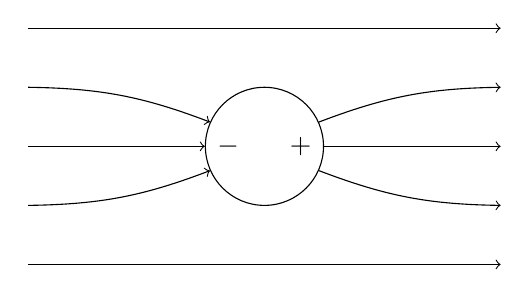
\begin{tikzpicture}
      \node [draw, circle, inner sep = 0, minimum size=1.5cm] (charge) {};
      \draw [->] (-3, 1.5) -- (3, 1.5);
      \draw [->] (-3, -1.5) -- (3, -1.5);
      \draw [<-] (charge) to [bend right=10] (-3, 0.75);
      \draw [<-] (charge) to [bend left=10] (-3, -0.75);
      \draw [->] (charge) to [bend left=10] (3, 0.75);
      \draw [->] (charge) to [bend right=10] (3, -0.75);
      \draw [->] (-3, 0) -- (charge);
      \draw [->] (charge) -- (3, 0);
      \node at (-0.2, 0) [left] {$-$};
      \node at (0.2, 0) [right] {$+$};
    \end{tikzpicture}
  \end{center}
  We get an induced surface charge.
\end{eg}

\begin{eg}
  Suppose we have a conductor that fills all space $x < 0$. We ground it such that $\phi = 0$ throughout the conductor. Then we place a charge $q$ at $x = d > 0$.
  \begin{center}
    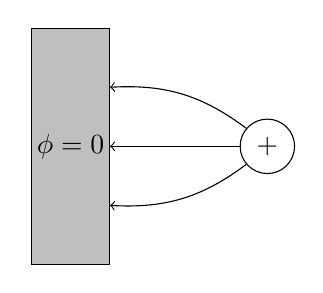
\begin{tikzpicture}
      \draw [fill=gray!50!white] (-1, 1.5) rectangle (0, -1.5);
      \node at (-0.5, 0) {$\phi = 0$};
      \node [draw, circle] (+) at (2, 0) {$+$};
      \draw [->] (+) -- (0, 0);
      \draw [->] (+) to [bend right=20] (0, 0.75);
      \draw [->] (+) to [bend left=20] (0, -0.75);
    \end{tikzpicture}
  \end{center}
  We are looking for a potential that corresponds to a source at $x = d$ and satisfies $\phi = 0$ for $x < 0$. Since the solution to the Poisson equation is unique, we can use the method of images to guess a solution and see if it works --- if it does, we are done.

  To guess a solution, we pretend that we don't have a conductor. Instead, we have a charge $-q$ and $x = -d$. Then by symmetry we will get $\phi = 0$ when $x = 0$. The potential of this pair is
  \[
    \phi = \frac{1}{4\pi\varepsilon_0}\left[\frac{q}{\sqrt{(x - d)^2 + y^2 + z^2}} - \frac{q}{\sqrt{(x + d)^2 + y^2 + z^2}}\right].
  \]
  To get the solution we want, we ``steal'' part of this potential and declare our potential to be
  \[
    \phi =
    \begin{cases}
      \frac{1}{4\pi\varepsilon_0}\left[\frac{q}{\sqrt{(x - d)^2 + y^2 + z^2}} - \frac{q}{\sqrt{(x + d)^2 + y^2 + z^2}}\right] & \text{if }x > 0\\
    0 & \text{if }x \leq 0
    \end{cases}
  \]
  Using this solution, we can immediately see that it satisfies Poisson's equations both outside and inside the conductor. To complete our solution, we need to find the surface charge required such that the equations are satisfied on the surface as well.

  To do so, we can calculate the electric field near the surface, and use the relation $\sigma = \varepsilon_0 \mathbf{E}_\text{outside}\cdot \hat{\mathbf{n}}$. To find $\sigma$, we only need the component of $\mathbf{E}$ in the $x$ direction:
  \[
    \mathbf{E}_x = -\frac{\partial \phi}{\partial x} = \frac{q}{4\pi\varepsilon_0}\left(\frac{x - d}{|\mathbf{r} - \mathbf{d}|^{3/2}} - \frac{x + d}{|\mathbf{r} + \mathbf{d}|^{3/2}}\right)
  \]
  for $x > 0$. Then induced surface charge density is given by $\mathbf{E}_x$ at $x = 0$:
  \[
    \sigma = E_x\varepsilon_0 = -\frac{q}{2\pi}\frac{d}{(d^2 + y^2 + z^2)^{3/2}}.
  \]
  The total surface charge is then given by
  \[
    \int \sigma \;\d y\;\d z = -q.
  \]
\end{eg}
\section{Magnetostatics}
Charges give rise to electric fields, currents give rise to magnetic fields. In this section, we study the magnetic fields induced by \emph{steady currents}, i.e.\ in situations where $\mathbf{J}\not= 0$ and $\rho = 0$. Again, we look for time-independent solutions.

Since there is no charge, we obtain $\mathbf{E} = 0$. The remaining Maxwell's equations are
\begin{align*}
  \nabla \times \mathbf{B} &= \mu \mathbf{J}\\
  \nabla\cdot \mathbf{B} &= 0
\end{align*}
The objective is, given a $\mathbf{J}$, find the resultant $\mathbf{B}$.

Before we start, what does the condition $\rho = 0$ mean? It does \emph{not} mean that there are no charges around. We want charges to be moving around to create current. What it means is that the positive and negative charges balance out exactly. More importantly, it stays that way. We don't have a net charge flow from one place to another. At any specific point in space, the amount of charge entering is the same as the amount of charge leaving. This is the case in many applications. For example, in a wire, all electrons move together at the same rate, and we don't have charge building up at parts of the circuit.

Mathematically, we can obtain the interpretation from the continuity equation:
\[
  \frac{\partial\rho}{\partial t} + \nabla \cdot \mathbf{J} = 0.
\]
In the case of steady currents, we have $\rho = 0$. So
\[
  \nabla\cdot \mathbf{J} = 0,
\]
which says that there is no net flow in or out of a point.
\subsection{Ampere's Law}
Consider a surface $S$ with boundary $C$. Current $\mathbf{J}$ flows through $S$. We now integrate the first equation over the surface $S$ to obtain
\[
  \int_S (\nabla\times \mathbf{B})\cdot \d S = \oint_C \mathbf{B}\cdot \d \mathbf{r} = \mu_0 \int_S \mathbf{J}\cdot \d S.
\]
So
\begin{law}[Ampere's law]
  \[
    \oint_C \mathbf{B}\cdot \d \mathbf{r} = \mu_0 I,
  \]
  where $I$ is the current through the surface.
\end{law}

\begin{eg}[A long straight wire]
  A wire is a cylinder with current $I$ flowing through it.

  We use cylindrical polar coordinates $(r, \varphi, z)$, where $z$ is along the direction of the current, and $r$ points in the radial direction.
  \begin{center}
    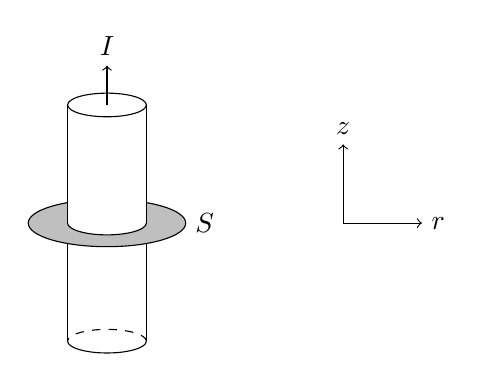
\begin{tikzpicture}
      \draw (0, 1.5) circle [x radius=0.5, y radius = 0.15];
      \draw [dashed] (0.5, -1.5) arc (0: 180:0.5 and 0.15);
      \draw (-0.5, -1.5) arc (180: 360:0.5 and 0.15);
      \draw (0.5, 1.5) -- (0.5, -1.5);
      \draw (-0.5, 1.5) -- (-0.5, -1.5);

      \draw [->] (0, 1.5) -- (0, 2) node [above] {$I$};

      \draw [fill = gray!50!white] circle [x radius = 1, y radius = 0.3];
      \draw [fill = white] circle [x radius = 0.5, y radius = 0.15];
      \draw [fill = white, draw = none] (-0.5, 0) rectangle (0.5, 1);
      \draw (-0.5, 0) -- (-0.5, 1);
      \draw (0.5, 0) -- (0.5, 1);
      \node at (1, 0) [right] {$S$};

      \draw [->] (3, 0) -- (3, 1) node [above] {$z$};
      \draw [->] (3, 0) -- (4, 0) node [right] {$r$};
    \end{tikzpicture}
  \end{center}
  By symmetry, the magnetic field can only depend on the radius, and must lie in the $x,y$ plane. Since we require that $\nabla\cdot \mathbf{B} = 0$, we cannot have a radial component. So the general form is
  \[
    \mathbf{B}(\mathbf{r}) = B(r)\hat{\boldsymbol\varphi}.
  \]
  To find $B(r)$, we integrate over a disc that cuts through the wire horizontally. We have
  \[
    \oint_C \mathbf{B}\cdot \d \mathbf{r} = B(r)\int_0^{2\pi} r\;\d \varphi = 2\pi r B(r)
  \]
  By Ampere's law, we have
  \[
    2\pi rB(r) = \mu_0 I.
  \]
  So
  \[
    \mathbf{B}(r) = \frac{\mu_0 I}{2\pi r} \hat{\boldsymbol\varphi}.
  \]
\end{eg}

\begin{eg}[Surface current]
  Consider the plane $z = 0$ with \emph{surface current density} $\mathbf{k}$ (i.e.\ current per unit length).
  \begin{center}
     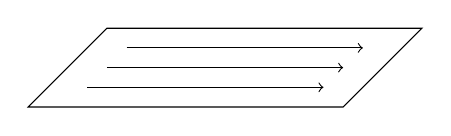
\begin{tikzpicture}[
        y = {(0.5cm,0.5cm)},
        z = {(0cm,1cm)}]
      \draw (-2, -1, 0) -- (2, -1, 0) -- (2, 1, 0) -- (-2, 1, 0) -- cycle;
      \draw [->] (-1.5, 0.5, 0) -- (1.5, 0.5, 0);
      \draw [->] (-1.5, -0.5, 0) -- (1.5, -0.5, 0);
      \draw [->] (-1.5, 0, 0) -- (1.5, 0, 0);
    \end{tikzpicture}
  \end{center}
  Take the x-direction to be the direction of the current, and the $z$ direction to be the normal to the plane.

  We imagine this situation by considering this to be infinitely many copies of the above wire situation. Then the magnetic fields must point in the $y$-direction. By symmetry, we must have
  \[
    \mathbf{B} = -B(z) \hat{\mathbf{y}},
  \]
  with $B(z) = -B(-z)$.

  Consider a vertical rectangular loop of length $L$ through the surface
  \begin{center}
    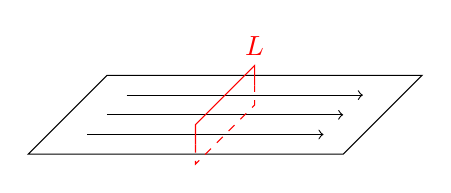
\begin{tikzpicture}[
        y = {(0.5cm,0.5cm)},
        z = {(0cm,1cm)}]
      \draw (-2, -1, 0) -- (2, -1, 0) -- (2, 1, 0) -- (-2, 1, 0) -- cycle;
      \draw [->] (-1.5, 0.5, 0) -- (1.5, 0.5, 0);
      \draw [->] (-1.5, -0.5, 0) -- (1.5, -0.5, 0);
      \draw [->] (-1.5, 0, 0) -- (1.5, 0, 0);
      \draw [red] (0, 0.75, 0) -- (0, 0.75, 0.25) node [above] {$L$} -- (0, -0.75, 0.25) -- (0, -0.75, 0);
      \draw [dashed, red] (0, -0.75, 0) -- (0, -0.75, -0.25) -- (0, 0.75, -0.25) -- (0, 0.75, 0);
    \end{tikzpicture}
  \end{center}
  Then
  \[
    \oint_C \mathbf{B}\cdot \d \mathbf{r} = LB(z) - LB(-z) = \mu_0 kL
  \]
  So
  \[
    B(z) = \frac{\mu_0 k}{2}\quad\text{ for }z > 0.
  \]
  Similar to the electrostatic case, the magnetic field is constant, and the part parallel to the surface is discontinuous across the plane. This is a general result, i.e.\ across any surface,
  \[
    \hat {\mathbf{n}} \times \mathbf{B}_+ - \hat{\mathbf{n}}\times \mathbf{B}_{-} = \mu_0 \mathbf{k}.
  \]
\end{eg}

\begin{eg}[Solenoid]
  A \emph{solenoid} is a cylindrical surface current, usually made by wrapping a wire around a cylinder.
  \begin{center}
    \begin{tikzpicture}
      \draw (0, 1.5) circle [x radius=0.5, y radius = 0.15];
      \draw [dashed] (0.5, -1.5) arc (0: 180:0.5 and 0.15);
      \draw (-0.5, -1.5) arc (180: 360:0.5 and 0.15);
      \draw [red, dashed] (0.5, -1) arc (0: 180:0.5 and 0.15);
      \draw [red, ->-=0.6] (-0.5, -1) arc (180: 360:0.5 and 0.15);
      \draw [red, dashed] (0.5, -0.5) arc (0: 180:0.5 and 0.15);
      \draw [red, ->-=0.6] (-0.5, -0.5) arc (180: 360:0.5 and 0.15);
      \draw [red, dashed] (0.5, 0) arc (0: 180:0.5 and 0.15);
      \draw [red, ->-=0.6] (-0.5, 0) arc (180: 360:0.5 and 0.15);
      \draw [red, dashed] (0.5, 0.5) arc (0: 180:0.5 and 0.15);
      \draw [red, ->-=0.6] (-0.5, 0.5) arc (180: 360:0.5 and 0.15);
      \draw [red, dashed] (0.5, 1) arc (0: 180:0.5 and 0.15);
      \draw [red, ->-=0.6] (-0.5, 1) arc (180: 360:0.5 and 0.15);
      \draw (0.5, 1.5) -- (0.5, -1.5);
      \draw (-0.5, 1.5) -- (-0.5, -1.5);

      \draw [->] (3, 0) -- (3, 1) node [above] {$z$};
      \draw [->] (3, 0) -- (4, 0) node [right] {$r$};

      \draw (0.2, 1) -- (0.8, 1) node[anchor = south west] {$C$};
      \draw [->-=0.6] (0.8, 1) -- (0.8, -1);
      \draw (0.8, -1) -- (0.2, -1) -- (0.2, 1);
    \end{tikzpicture}
  \end{center}
  We use cylindrical polar coordinates with $z$ in the direction of the extension of the cylinder. By symmetry, $\mathbf{B} = B(r)\hat{\mathbf{z}}$.

  Away from the cylinder, $\nabla \times \mathbf{B} = 0$. So $\frac{\partial B}{\partial r} = 0$, which means that $B(r)$ is constant outside. Since we know that $\mathbf{B} = \mathbf{0}$ at infinity, $\mathbf{B} = \mathbf{0}$ everywhere outside the cylinder.

  To compute $\mathbf{B}$ inside, use Ampere's law with a curve $C$. Note that only the vertical part (say of length $L$) inside the cylinder contributes to the integral. Then
  \[
    \oint_C \mathbf{B}\cdot \d \mathbf{r} = BL = \mu_o INL.
  \]
  where $N$ is the number of wires per unit length and $I$ is the current in each wire (so $INL$ is the total amount of current through the wires).

  So
  \[
    B = \mu_0 IN.
  \]
\end{eg}

\subsection{Vector potential}
For general current distributions $\mathbf{J}$, we also need to solve $\nabla \cdot \mathbf{B} = 0$.

Recall that for the electric case, the equation is $\nabla\cdot \mathbf{E} = \rho/\varepsilon_0$. For the $\mathbf{B}$ field, we have $0$ on the right hand side instead of $\rho/\varepsilon_0$. This is telling us that there are no magnetic monopoles, i.e.\ magnetic charges.

The general solution to this equation is $\mathbf{B} = \nabla \times \mathbf{A}$ for some $\mathbf{A}$.
\begin{defi}[Vector potential]
  If $\mathbf{B} = \nabla\times \mathbf{A}$, then $\mathbf{A}$ is the \emph{vector potential}.
\end{defi}
The other Maxwell equation then says
\[
  \nabla \times \mathbf{B} = -\nabla^2 \mathbf{A} + \nabla(\nabla\cdot \mathbf{A}) = \mu_0 \mathbf{J}.\tag{$*$}
\]
This is rather difficult to solve, but it can be made easier by noting that $\mathbf{A}$ is not unique. If $\mathbf{A}$ is a vector potential, then for any function $\chi(\mathbf{x})$,
\[
  \mathbf{A}' = \mathbf{A} + \nabla \chi
\]
is also a vector potential of $\mathbf{B}$, since $\nabla \times (\mathbf{A} + \nabla \chi) = \nabla \times \mathbf{A}$.

The transformation $\mathbf{A} \mapsto \mathbf{A} + \nabla\chi$ is called a \emph{gauge transformation}.

\begin{defi}[(Coulomb) gauge]
  Each choice of $\mathbf{A}$ is called a \emph{gauge}. An $\mathbf{A}$ such that $\nabla \cdot \mathbf{A} = 0$ is called a \emph{Coulomb gauge}.
\end{defi}

\begin{prop}
  We can always pick $\chi$ such that $\nabla \cdot \mathbf{A}' = 0$.
\end{prop}

\begin{proof}
  Suppose that $\mathbf{B} = \nabla \times \mathbf{A}$ with $\nabla \cdot \mathbf{A} = \psi(\mathbf{x})$. Then for any $\mathbf{A}' = \mathbf{A} + \nabla \chi$, we have
  \[
    \nabla \cdot \mathbf{A}' = \nabla \mathbf{A} + \nabla^2 \chi = \psi + \nabla^2\chi.
  \]
  So we need a $\chi$ such that $\nabla^2\chi = -\psi$. This is the Poisson equation which we know that there is always a solution by, say, the Green's function. Hence we can find a $\chi$ that works.
\end{proof}

If $\mathbf{B} = \nabla\times \mathbf{A}$ and $\nabla\cdot \mathbf{A} = 0$, then the Maxwell equation $(*)$ becomes
\[
  \nabla^2 \mathbf{A} = -\mu_0 \mathbf{J}.
\]
Or, in Cartesian components,
\[
  \nabla^2 A_i = -\mu_0 J_i.
\]
This is 3 copies of the Poisson equation, which we know how to solve using Green's functions. The solution is
\[
  A_i (\mathbf{r}) = \frac{\mu_0}{4\pi}\int \frac{J_i (\mathbf{r}')}{|\mathbf{r} - \mathbf{r}'|}\;\d V',
\]
or
\[
  \mathbf{A}(\mathbf{r}) = \frac{\mu_0}{4\pi}\int \frac{\mathbf{J}(\mathbf{r'})}{|\mathbf{r} - \mathbf{r}'|}\;\d V',
\]
both integrating over $\mathbf{r}'$.

We have randomly written down a solution of $\nabla^2 \mathbf{A} = -\mu_0 \mathbf{J}$. However, this is a solution to Maxwell's equations only if it is a \emph{Coulomb gauge}. Fortunately, it is:
\begin{align*}
  \nabla\cdot \mathbf{A}(\mathbf{r}) &= \frac{\mu_0}{4\pi}\int \mathbf{J}(\mathbf{r}')\cdot \nabla\left(\frac{1}{|\mathbf{r} - \mathbf{r}'|}\right)\;\d V'\\
  &= -\frac{\mu_0}{4\pi}\int \mathbf{J}(\mathbf{r}') \cdot \nabla'\left(\frac{1}{|\mathbf{r} - \mathbf{r}'|}\right)\;\d V'\\
  \intertext{Here we employed a clever trick --- differentiating $1/|\mathbf{r} - \mathbf{r}'|$ with respect to $\mathbf{r}$ is the negative of differentiating it with respect to $\mathbf{r}'$. Now that we are differentiating against $\mathbf{r}'$, we can integrate by parts to obtain}
  &= -\frac{\mu_0}{4\pi}\int \left[\nabla'\cdot \left(\frac{\mathbf{J}(\mathbf{r}')}{|\mathbf{r} - \mathbf{r}'|}\right) - \frac{\nabla'\cdot \mathbf{J}(\mathbf{r}')}{|\mathbf{r} - \mathbf{r}'|}\right]\;\d V'.
\end{align*}
Here both terms vanish. We assume that the current is localized in some region of space so that $\mathbf{J} = \mathbf{0}$ on the boundary. Then the first term vanishes since it is a total derivative. The second term vanishes since we assumed that the current is steady ($\nabla\cdot \mathbf{J} = 0$). Hence we have Coulomb gauge.

\begin{law}[Biot-Savart law]
  The magnetic field is
  \[
    \mathbf{B}(\mathbf{r}) = \nabla \times \mathbf{A} = \frac{\mu_0}{4\pi}\int \mathbf{J}(\mathbf{r}')\times \frac{\mathbf{r} - \mathbf{r}'}{|\mathbf{r} - \mathbf{r}'|^3}\;\d V'.
  \]
  If the current is localized on a curve, this becomes
  \[
    \mathbf{B} = \frac{\mu_0 I}{4\pi}\oint_C \d \mathbf{r}' \times \frac{\mathbf{r} - \mathbf{r}'}{|\mathbf{r} - \mathbf{r}'|^3},
  \]
  since $\mathbf{J}(\mathbf{r}')$ is non-zero only on the curve.
\end{law}

\subsection{Magnetic dipoles}
According to Maxwell's equations, magnetic monopoles don't exist. However, it turns out that a localized current looks like a dipole from far far away.

\begin{eg}[Current loop]
  Take a current loop of wire $C$, radius $R$ and current $I$.
  \begin{center}
    \begin{tikzpicture}
      \clip (-2.1, 1.2) rectangle (2.1, -1.2);
      \draw [->-=0.8] circle [x radius = 1, y radius = 0.5];
      \draw [->, gray!70!black] (-1, 0) circle [x radius=0.4, y radius = 0.5];
      \draw [->, gray!70!black] (-1.2, 0) circle [x radius=0.8, y radius = 1.1];
      \draw [->, gray!70!black] (-1.3, 0) circle [x radius=1.1, y radius = 2];
      \draw [->-=0.5, gray!70!black] (0, -1.2) -- (0, 1.2);
      \draw [gray!70!black] (1, 0) circle [x radius=0.4, y radius = 0.5];
      \draw [gray!70!black] (1.2, 0) circle [x radius=0.8, y radius = 1.1];
      \draw [gray!70!black] (1.3, 0) circle [x radius=1.1, y radius = 2];
      \draw [gray!70!black, ->] (0.6, -0.01) -- (0.6, 0);
      \draw [gray!70!black, ->] (0.4, -0.01) -- (0.4, 0);
      \draw [gray!70!black, ->] (0.2, -0.01) -- (0.2, 0);
    \end{tikzpicture}
  \end{center}
  Based on the fields generated by a straight wire, we can guess that $\mathbf{B}$ looks like this, but we want to calculate it.

  By the Biot-Savart law, we know that
  \[
    \mathbf{A}(\mathbf{r}) = \frac{\mu_0}{4\pi}\int\frac{\mathbf{J}(\mathbf{r}')}{|\mathbf{r}-\mathbf{r}'|}\;\d V = \frac{\mu_0 I}{4\pi}\oint_C \frac{\d \mathbf{r}'}{|\mathbf{r} - \mathbf{r}'|}.
  \]
  Far from the loop, $|\mathbf{r} - \mathbf{r}'|$ is small and we can use the Taylor expansion.
  \[
    \frac{1}{|\mathbf{r} - \mathbf{r}'|} = \frac{1}{r} + \frac{\mathbf{r}\cdot \mathbf{r}'}{r^3} + \cdots
  \]
  Then
  \[
    \mathbf{A}(\mathbf{r}) = \frac{\mu_0 I}{4\pi}\oint_C \left(\frac{1}{r} + \frac{\mathbf{r}\cdot \mathbf{r}'}{r^3} + \cdots\right) \d \mathbf{r}'.
  \]
  Note that $r$ is a constant of the integral, and we can take it out. The first $\frac{1}{r}$ term vanishes because it is a constant, and when we integrate along a closed loop, we get 0. So we only consider the second term.

  We claim that for any constant vector $\mathbf{g}$,
  \[
    \oint_C \mathbf{g}\cdot \mathbf{r}' \;\d \mathbf{r}' = \mathbf{S}\times \mathbf{g},
  \]
  where $\mathbf{S} = \int \d \mathbf{\mathbf{S}}$ is the \emph{vector area} of the surface bounded by $C$. It follows from Green's theorem for the function $f(r')$:
  \[
    \oint_C f(r')\d \mathbf{r}' = \int_S \nabla f\times\d \mathbf{S},
  \]
  taking $f(r') = \mathbf{g}\cdot \mathbf{r}'$. Then
  \[
    \oint_C \mathbf{g}\cdot \mathbf{r}'\;\d \mathbf{r}' = \int_S \mathbf{g}\times \d \mathbf{S} = \mathbf{S}\times \mathbf{g}.
  \]
  Using this, we have
  \[
    \mathbf{A}(\mathbf{r}) \approx \frac{\mu_0}{4\pi}\frac{\mathbf{m}\times \mathbf{r}}{r^3},
  \]
  where
  \begin{defi}[Magnetic dipole moment] The \emph{magnetic dipole moment} is
    \[
      \mathbf{m} = I\mathbf{S}.
    \]
  \end{defi}
  Then
  \[
    \mathbf{B} = \nabla\times \mathbf{A} = \frac{\mu_0}{4\pi}\left(\frac{3(\mathbf{m}\cdot \hat{\mathbf{r}})\hat{\mathbf{r}} - \mathbf{m}}{r^3}\right).
  \]
  This is the same form as $\mathbf{E}$ for an electric dipole, except that there is no $1/r^2$ leading term here, because we have no magnetic monopoles.
\end{eg}

After doing it for a loop, we can do it for a general current distribution:
\begin{eg}
  We have
  \begin{align*}
    A_i(\mathbf{r}) &= \frac{\mu_0}{4\pi}\int \frac{J_i(\mathbf{r}')}{|\mathbf{r} - \mathbf{r}'|}\;\d V'\\
    &= \frac{\mu_0}{4\pi}\int\left(\frac{J_i(\mathbf{r}')}{r} - \frac{J_i(\mathbf{r}')(\mathbf{r}\cdot \mathbf{r}')}{r^3} + \cdots\right)\;\d V'.
  \end{align*}
  We will show that the first term vanishes by showing that it is a total derivative. We have
  \[
    \partial_j'(J_jr_i') = \underbrace{(\partial_j'J_j)}_{=\nabla\cdot \mathbf{J} = 0}r_i' + \underbrace{(\partial_j'r_i')}_{=\delta_{ij}}J_j = J_i.
  \]
  For the second term, we look at
  \[
    \partial_j' (J_jr_i'r_k') = (\partial_j'J_j)r_i'r_k' + J_ir_k' + J_kr_i' =J_kr_i' + J_ir_k'.
  \]
  Apply this trick to
  \[
    \int J_ir_jr'_j \;\d V = \int \frac{r_j}{2}(J_i r_j' - J_j r'_i)\;\d V',
  \]
  where we discarded a total derivative $\partial_j'(J_jr_i'r_u')$. Putting it back in vector notation,
  \begin{align*}
    \int J_i\mathbf{r}\cdot \mathbf{r}'\;\d V &= \int\frac{1}{2}\left(J_i(\mathbf{r}\cdot \mathbf{r}') - r_i(\mathbf{J}\cdot \mathbf{r}')\right)\;\d V\\
    &= \int \frac{1}{2}\left[\mathbf{r}\times (\mathbf{J}\times \mathbf{r}')\right]_i\;\d V.
  \end{align*}
  So the long-distance vector potential is again
  \[
    \mathbf{A} (\mathbf{r}) = \frac{\mu_0}{4\pi}\frac{\mathbf{m}\times \mathbf{r}}{r^3},
  \]
  with
  \begin{defi}[Magnetic dipole moment]
    \[
      \mathbf{m} = \frac{1}{2}\int \mathbf{r}'\times \mathbf{J}(\mathbf{r}')\;\d V'.
    \]
  \end{defi}
\end{eg}

\subsection{Magnetic forces}
We've seen that moving charge produces currents which generates a magnetic field. But we also know that a charge moving in a magnetic field experiences a force $\mathbf{F} = q\mathbf{r}\times \mathbf{B}$. So two currents will exert a force on each other.

\begin{eg}[Two parallel wires]\leavevmode
  \begin{center}
    \begin{tikzpicture}
      \draw [->-=0.5] (-1, -2) -- (-1, 2);
      \draw [->-=0.5] (1, -2) -- (1, 2);
      \draw [->] (-1, -1.5) -- (1, -1.5) node [pos = 0.5, below] {$d$};
      \draw [->] (1, -1.5) -- (-1, -1.5);

      \draw [->] (3, 0) -- (3, 1) node [above] {$z$};
      \draw [->] (3, 0) -- (4, 0) node [right] {$x$};
      \draw [->] (3, 0) -- (3.8, 0.6) node [anchor = south west] {$y$};
    \end{tikzpicture}
  \end{center}
  We know that the field produced by each current is
  \[
    \mathbf{B}_1 = \frac{\mu_0 I}{2\pi r}\hat{\varphi}.
  \]
  The particles on the second wire will feel a force
  \[
    \mathbf{F} = q\mathbf{v}\times \mathbf{B}_1 = q\mathbf{v}\times \left(\frac{\mu_0 I_1}{2\pi d}\right) \hat{\mathbf{y}}.
  \]
  But $\mathbf{J}_2 = nq\mathbf{v}$ and $I_2 = J_2 A$, where $n$ is the density of particles and $A$ is the cross-sectional area of the wire. So the number of particles per unit length is $nA$, and the force per unit length is
  \[
    nA\mathbf{F} = \frac{\mu_0 I_1I_2}{2\pi d}\hat{\mathbf{z}}\times \hat{\mathbf{y}} = -\mu_0\frac{I_1I_2}{2\pi d}\hat{\mathbf{x}}.
  \]
  So if $I_1I_2 > 0$, i.e.\ the currents are in the same direction, the force is attractive. Otherwise the force is repulsive.
\end{eg}

\begin{eg}[General force]
  A current $\mathbf{J}_1$, localized on some closed curve $C_1$, sets up a magnetic field
  \[
    \mathbf{B}(\mathbf{r}) = \frac{\mu_0I_1}{4\pi}\oint_{C_1} \d \mathbf{r}_1 \times \frac{\mathbf{r} - \mathbf{r}_1}{|\mathbf{r} - \mathbf{r}_1|^3}.
  \]
  A second current $\mathbf{J}_2$ on $C_2$ experiences the Lorentz force
  \[
    \mathbf{F} = \int \mathbf{J}_2(\mathbf{r})\times \mathbf{B}(\mathbf{r})\;\d V.
  \]
  While we are integrating over all of space, the current is localized at a curve $C_2$. So
  \[
    \mathbf{F} = I_2\oint_{C_2} \d \mathbf{r}_2 \times \mathbf{B}(\mathbf{r}_2).
  \]
  Hence
  \[
    \mathbf{F} = \frac{\mu_0}{4\pi} I_1 I_2 \oint_{C_1}\oint_{C_2}\d \mathbf{r}_2\times \left(\d \mathbf{r}_1\times \frac{\mathbf{r}_2 - \mathbf{r}_1}{|\mathbf{r}_2 - \mathbf{r}_1|^3}\right).
  \]
  For well-separated currents, approximated by $\mathbf{m}_1$ and $\mathbf{m}_2$, we claim that the force can be written as
  \[
    \mathbf{F} = \frac{\mu_0}{4\pi}\nabla\left(\frac{3(\mathbf{m}_1\cdot \hat{\mathbf{r}})(\mathbf{m}_2\cdot \hat{\mathbf{r}}) - (\mathbf{m}_1\cdot \mathbf{m}_2)}{r^3}\right),
  \]
  whose proof is too complicated to be included.
\end{eg}

Note that we've spent a whole chapter discussing ``magnets'', but they are nothing like what we stick on our fridges. It turns out that these ``real'' magnets are composed of many tiny aligned microscopic dipoles arising from electron spin. However, obviously we do not care about magnets in real life.

\section{Electrodynamics}
So far, we have only looked at fields that do not change with time. However, in real life, fields \emph{do} change with time. We will now look at time-dependent $\mathbf{E}$ and $\mathbf{B}$ fields.
\subsection{Induction}
We'll explore the Maxwell equation
\[
  \nabla\times \mathbf{E} + \frac{\partial \mathbf{B}}{\partial t} = 0.
\]
In short, if the magnetic field changes in time, i.e.\ $\frac{\partial \mathbf{B}}{\partial t} \not = 0$, this creates an $\mathbf{E}$ that accelerates charges, which creates a current in a wire. This process is called induction. Consider a wire, which is a closed curve $C$, with a surface $S$.

We integrate over the surface $S$ to obtain
\[
  \int_S (\nabla\times \mathbf{E})\cdot \d \mathbf{S} = -\int_S \frac{\partial \mathbf{B}}{\partial t}\cdot \d \mathbf{S}.
\]
By Stokes' theorem and commutativity of integration and differentiation (assuming $S$ and $C$ do not change in time), we have
\[
  \int_C \mathbf{E}\cdot \d \mathbf{r} = - \frac{\d }{\d t} \int _S \mathbf{B} \cdot \d \mathbf{S}.
\]
\begin{defi}[Electromotive force (emf)]
  The \emph{electromotive force} (emf) is
  \[
    \mathcal{E} = \int_C \mathbf{E}\cdot \d \mathbf{r}.
  \]
  Despite the name, this is not a force! We can think of it as the work done on a unit charge moving around the curve, or the ``voltage'' of the system.
\end{defi}

For convenience we define the quantity
\begin{defi}[Magnetic flux]
  The \emph{magnetic flux} is
  \[
    \Phi = \int_S \mathbf{B}\cdot \d \mathbf{S}.
  \]
\end{defi}
Then we have
\begin{law}[Faraday's law of induction]
  \[
    \mathcal{E} = -\frac{\d \Phi}{\d t}.
  \]
\end{law}
This says that when we change the magnetic flux through $S$, then a current is induced. In practice, there are many ways we can change the magnetic flux, such as by moving bar magnets or using an electromagnet and turning it on and off.

The minus sign has a significance. When we change a magnetic field, an emf is created. This induces a current around the wire. However, we also know that currents produce magnetic fields. The minus sign indicates that the induced magnetic field \emph{opposes} the initial change in magnetic field. If it didn't and the induced magnetic field reinforces the change, we will get runaway behaviour and the world will explode. This is known as \emph{Lenz's law}.

\begin{eg}
  Consider a circular wire with a magnetic field perpendicular to it.
  \begin{center}
    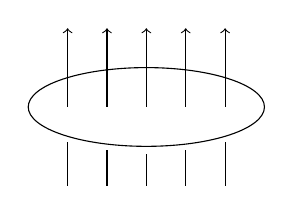
\begin{tikzpicture}
      \draw circle [x radius = 1.5, y radius = 0.5];
      \draw [->] (0, 0) -- (0, 1);
      \draw [->] (-0.5, 0) -- (-0.5, 1);
      \draw [->] (-1, 0) -- (-1, 1);
      \draw [->] (0.5, 0) -- (0.5, 1);
      \draw [->] (1, 0) -- (1, 1);
      \draw (0, -0.6) -- (0, -1);
      \draw (0.5, -0.55) -- (0.5, -1);
      \draw (1, -0.45) -- (1, -1);
      \draw (-0.5, -0.55) -- (-0.5, -1);
      \draw (-1, -0.45) -- (-1, -1);
    \end{tikzpicture}
  \end{center}
  If we decrease $\mathbf{B}$ such that $\dot{\Phi} < 0$, then $\mathcal{E} > 0$. So the current flows anticlockwise (viewed from above). The current generates its own $\mathbf{B}$. This acts to \emph{increase} $\mathbf{B}$ inside, which counteracts the initial decrease.
  \begin{center}
    \begin{tikzpicture}[xscale = 2]
      \clip (-2.1, 1.2) rectangle (2.1, -1.2);
      \draw [->-=0.8] circle [x radius = 1, y radius = 0.5];
      \draw [->, gray!50!black] (-1, 0) circle [x radius=0.4, y radius = 1];
      \draw [->, gray!50!black] (-1.2, 0) circle [x radius=0.8, y radius = 2.2];
      \draw [->, gray!50!black] (-1.3, 0) circle [x radius=1.1, y radius = 4];
      \draw [->-=0.5, gray!50!black] (0, -1.2) -- (0, 1.2);
      \draw [gray!50!black] (1, 0) circle [x radius=0.4, y radius = 1];
      \draw [gray!50!black] (1.2, 0) circle [x radius=0.8, y radius = 2.2];
      \draw [gray!50!black] (1.3, 0) circle [x radius=1.1, y radius = 4];
      \draw [gray!50!black, ->] (0.6, -0.01) -- (0.6, 0);
      \draw [gray!50!black, ->] (0.4, -0.01) -- (0.4, 0);
      \draw [gray!50!black, ->] (0.2, -0.01) -- (0.2, 0);
    \end{tikzpicture}
  \end{center}
  This means you don't get runaway behaviour.
\end{eg}
There is a related way to induce a current: keep $\mathbf{B}$ fixed and move wire.

\begin{eg}\leavevmode
  \begin{center}
    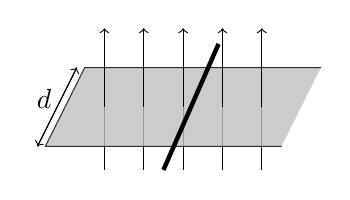
\begin{tikzpicture}
      \draw [->] (0.4, 1) -- (-0.1, 0) node [pos = 0.4, left] {$d$};
      \draw [->] (-0.1, 0) -- (0.4, 1);
      \draw (0.75, 0.5) -- (0.75, -0.3);
      \draw (1.25, 0.5) -- (1.25, -0.3);
      \draw (1.75, 0.5) -- (1.75, -0.3);
      \draw (2.25, 0.5) -- (2.25, -0.3);
      \draw (2.75, 0.5) -- (2.75, -0.3);

      \draw [fill=gray!50!white, opacity=0.8] (3, 0) -- (0, 0) -- (0.5, 1) -- (3.5, 1);
      \draw [ultra thick] (1.5, -0.3) -- (2.2, 1.3);

      \draw [->] (0.75, 0.5) -- (0.75, 1.5);
      \draw [->] (1.25, 0.5) -- (1.25, 1.5);
      \draw [->] (1.75, 0.5) -- (1.75, 1.5);
      \draw [->] (2.25, 0.5) -- (2.25, 1.5);
      \draw [->] (2.75, 0.5) -- (2.75, 1.5);
    \end{tikzpicture}
  \end{center}
  Slide the bar to the left with speed $v$. Each charge $q$ will experience a Lorentz force
  \[
    F = qvB,
  \]
  in the counterclockwise direction.

  The emf, defined as the work done per unit charge, is
  \[
    \mathcal{E} = vBd,
  \]
  because work is only done for particles on the bar.

  Meanwhile, the change of flux is
  \[
    \frac{\d \Phi}{\d t} = -vBd,
  \]
  since the area decreases at a rate of $-vd$.

  We again have
  \[
    \mathcal{E} = -\frac{\d \Phi}{\d t}.
  \]
  Note that we obtain the same formula but different physics --- we used Lorentz force law, not Maxwell's equation.
\end{eg}

Now we consider the general case: a moving loop $C(t)$ bounding a surface $S(t)$. As the curve moves, the curve sweeps out a cylinder $S_c$.
\begin{center}
  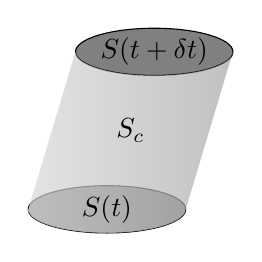
\begin{tikzpicture}
    \draw [fill=gray] circle [x radius=1cm, y radius=0.3cm];
    \draw [fill=gray] (0.6, 2) circle [x radius=1cm, y radius=0.3cm] node {$S(t + \delta t)$};
    \shade [left color=gray!30!white, right color=gray!70!white, opacity=0.7] (-1, 0) arc (180:360:1 and 0.3) -- (1.6, 2) arc (360:180:1 and 0.3) -- (-1, 0);

    \node {$S(t)$};
    \node at (0.3, 1) {$S_c$};
  \end{tikzpicture}
\end{center}
The change in flux
\begin{align*}
  \Phi(t + \delta t) - \Phi(t) &= \int_{S(t + \delta t)} \mathbf{B}(t + \delta t)\cdot \d \mathbf{S} - \int_{S(t)}\mathbf{B}(t)\cdot \d \mathbf{S}\\
  &= \int_{S(t + \delta t)}\left(\mathbf{B}(t) + \frac{\partial \mathbf{B}}{\partial t}\right)\cdot \d \mathbf{S} - \int_{S(t)}\mathbf{B}(t)\cdot \d \mathbf{S} + O(\delta t^2)\\
  &= \delta t\int_{S(t)}\frac{\partial \mathbf{B}}{\partial t}\cdot \d \mathbf{S} + \left[\int_{S(t + \delta t)} - \int_{S(t)}\right]\mathbf{B}(t)\cdot \d \mathbf{S} + O(\delta t^2)
\end{align*}
We know that $S(t + \delta t)$, $S(t)$ and $S_c$ together form a closed surface. Since $\nabla\cdot \mathbf{B} = 0$, the integral of $\mathbf{B}$ over a closed surface is $0$. So we obtain
\[
  \left[\int_{S(t + \delta t)} - \int_{S(t)}\right]\mathbf{B}(t)\cdot \d \mathbf{S} + \int_{S_c}\mathbf{B}(t)\cdot \d \mathbf{S} = 0.
\]
Hence we have
\[
  \Phi(t + \delta t) - \Phi(t) = \delta t\int_{S(t)}\frac{\partial \mathbf{B}}{\partial t}\cdot \d \mathbf{S} - \int_{S_c}\mathbf{B}(t)\cdot \d \mathbf{S} = 0.
\]
We can simplify the integral over $S_c$ by writing the surface element as
\[
  \d \mathbf{S} = (\d \mathbf{r}\times \mathbf{v})\;\delta t.
\]
Then $\mathbf{B}\cdot \d \mathbf{S} = \delta t(\mathbf{v}\times \mathbf{B}) \cdot \d \mathbf{r}$. So
\[
  \frac{\d \Phi}{\d t} = \lim_{\delta \to 0}\frac{\delta \Phi}{\delta t} = \int_{S(t)}\frac{\partial \mathbf{B}}{\partial t}\cdot \d \mathbf{S} - \int_{C(t)}(\mathbf{v}\times \mathbf{B})\cdot \d \mathbf{r}.
\]
From Maxwell's equation, we know that $\frac{\partial \mathbf{B}}{\partial t} = -\nabla \times \mathbf{E}$. So we have
\[
  \frac{\d \Phi}{\d t} = -\int_C (\mathbf{E} + \mathbf{v}\times \mathbf{B})\;\d \mathbf{r}.
\]
Defining the emf as
\[
  \mathcal{E} = \int_C (\mathbf{E} + \mathbf{v}\times \mathbf{B})\;\d \mathbf{r},
\]
we obtain the equation
\[
  \mathcal{E} = -\frac{\partial \Phi}{\partial t}
\]
for the most general case where the curve itself can change.
\subsection{Magnetostatic energy}
Suppose that a current $I$ flows along a wire $C$. From magnetostatics, we know that this gives rise to a magnetic field $\mathbf{B}$, and hence a flux $\Phi$ given by
\[
  \Phi = \int_S \mathbf{B}\cdot \d \mathbf{S},
\]
where $S$ is the surface bounded by $C$.
\begin{defi}[Inductance]
  The \emph{inductance} of a curve $C$, defined as
  \[
    L = \frac{\Phi}{I},
  \]
  is the amount of flux it generates per unit current passing through $C$. This is a property only of the curve $C$.
\end{defi}

Inductance is something engineers care a \emph{lot} about, as they need to create real electric circuits and make things happen. However, us mathematicians find these applications completely pointless and don't actually care about inductance. The only role it will play is in the proof we perform below.

\begin{eg}[The solenoid]
  Consider a solenoid of length $\ell$ and cross-sectional area $A$ (with $\ell \gg \sqrt{A}$ so we can ignore end effects). We know that
  \[
    B = \mu_0 IN,
  \]
  where $N$ is the number of turns of wire per unit length and $I$ is the current. The flux through a single turn (pretending it is closed) is
  \[
    \Phi_0 = \mu_0 INA.
  \]
  So the total flux is
  \[
    \Phi = \Phi_0 N\ell = \mu_0 IN^2V,
  \]
  where $V$ is the volume, $A\ell$. So
  \[
    L = \mu_0 N^2 V.
  \]
\end{eg}

We can use the idea of inductance to compute the energy stored in magnetic fields. The idea is to compute the work done in building up a current.

As we build the current, the change in current results in a change in magnetic field. This produces an induced emf that we need work to oppose. The emf is given by
\[
  \mathcal{E} = -\frac{\d \Phi}{\d t} = -L\frac{\d I}{\d t}.
\]
This opposes the change in current by Lenz's law. In time $\delta t$, a charge $I\delta t$ flows around $C$. The work done is
\[
  \delta W = \mathcal{E} I\delta t = -LI\frac{\d I}{\d t}\delta t.
\]
So
\[
  \frac{\d W}{\d t} = -LI \frac{\d I}{\d t} = -\frac{1}{2}L\frac{\d I^2}{\d t}.
\]
So the work done to build up a current is
\[
  W = \frac{1}{2}LI^2 = \frac{1}{2}I\Phi.
\]
Note that we dropped the minus sign because we switched from talking about the work done by the emf to the work done to oppose the emf.

This work done is identified with the energy stored in the system. Recall that the vector potential $\mathbf{A}$ is given by $\mathbf{B} = \nabla \times \mathbf{A}$. So
\begin{align*}
  U &= \frac{1}{2}I\int_S \mathbf{B}\cdot \d \mathbf{S}\\
  &= \frac{1}{2}I\int_S(\nabla\times \mathbf{A})\cdot \d \mathbf{S}\\
  &= \frac{1}{2}I\oint_C \mathbf{A}\cdot \d \mathbf{r}\\
  &= \frac{1}{2}\int_{\R^3} \mathbf{J}\cdot \mathbf{A}\;\d V\\
  \intertext{Using Maxwell's equation $\nabla\times \mathbf{B} = \mu_0 \mathbf{J}$, we obtain}
  &= \frac{1}{2\mu_0}\int (\nabla\times \mathbf{B})\cdot \mathbf{A}\;\d V\\
  &= \frac{1}{2\mu_0}\int[\nabla\cdot(\mathbf{B}\times \mathbf{A}) + \mathbf{B}\cdot (\nabla\times \mathbf{A})]\;\d V\\
  \intertext{Assuming that $\mathbf{B}\times \mathbf{A}$ vanishes sufficiently fast at infinity, the integral of the first term vanishes. So we are left with}
  &= \frac{1}{2\mu_0}\int \mathbf{B}\cdot \mathbf{B}\;\d V.
\end{align*}
So
\begin{prop}
  The energy stored in a magnetic field is
  \[
    U = \frac{1}{2\mu_0}\int \mathbf{B}\cdot \mathbf{B}\;\d V.
  \]
\end{prop}
In general, the energy stored in $\mathbf{E}$ and $\mathbf{B}$ is
\[
  U = \int \left(\frac{\varepsilon_0}{2}\mathbf{E}\cdot \mathbf{E} + \frac{1}{2\mu_0}\mathbf{B}\cdot \mathbf{B}\right)\;\d V.
\]
Note that while this is true, it does not follow directly from our results for pure magnetic and pure electric fields. It is entirely plausible that when both are present, they interact in weird ways that increases the energy stored. However, it turns out that this does not happen, and this formula is right.

\subsection{Resistance}
The story so far is that we change the flux, an emf is produced, and charges are accelerated. In principle, we should be able to compute the current. But accelerating charges are complicated (they emit light). Instead, we invoke a new effect, friction.

In a wire, this is called \emph{resistance}. In most materials, the effect of resistance is that $\mathcal{E}$ is proportional to the speed of the charged particles, rather than the acceleration.

We can think of the particles as accelerating for a very short period of time, and then reaching a terminal velocity. So
\begin{law}[Ohm's law]
  \[
    \mathcal{E} = IR,
  \]
\end{law}
\begin{defi}[Resistance]
  The \emph{resistance} is the $R$ in Ohm's law.
\end{defi}
Note that $\mathcal{E} = \int \mathbf{E}\cdot \d \mathbf{r}$ and $\mathbf{E} = - \nabla\phi$. So $\mathcal{E} = V$, the potential difference. So Ohm's law can also be written as $V = IR$.

\begin{defi}[Resistivity and conductivity]
For the wire of length $L$ and cross-sectional area $A$, we define the \emph{resistivity} to be
\[
  \rho = \frac{AR}{L},
\]
and the conductivity is
\[
  \sigma = \frac{1}{\rho}.
\]
\end{defi}
These are properties only of the substance and not the actual shape of the wire. Then Ohm's law reads
\begin{law}[Ohm's law]
  \[
    \mathbf{J} = \sigma \mathbf{E}.
  \]
\end{law}
We can formally derive Ohm's law by considering the field and interactions between the electron and the atoms, but we're not going to do that.

\begin{eg}\leavevmode
  \begin{center}
    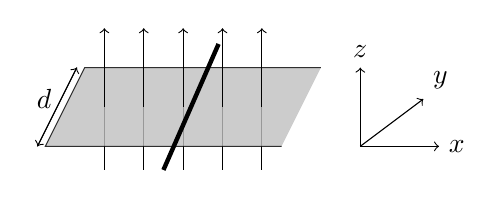
\begin{tikzpicture}
      \draw [->] (0.4, 1) -- (-0.1, 0) node [pos = 0.4, left] {$d$};
      \draw [->] (-0.1, 0) -- (0.4, 1);
      \draw (0.75, 0.5) -- (0.75, -0.3);
      \draw (1.25, 0.5) -- (1.25, -0.3);
      \draw (1.75, 0.5) -- (1.75, -0.3);
      \draw (2.25, 0.5) -- (2.25, -0.3);
      \draw (2.75, 0.5) -- (2.75, -0.3);

      \draw [fill=gray!50!white, opacity=0.8] (3, 0) -- (0, 0) -- (0.5, 1) -- (3.5, 1);
      \draw [ultra thick] (1.5, -0.3) -- (2.2, 1.3);

      \draw [->] (0.75, 0.5) -- (0.75, 1.5);
      \draw [->] (1.25, 0.5) -- (1.25, 1.5);
      \draw [->] (1.75, 0.5) -- (1.75, 1.5);
      \draw [->] (2.25, 0.5) -- (2.25, 1.5);
      \draw [->] (2.75, 0.5) -- (2.75, 1.5);

      \draw [->] (4, 0) -- (4, 1) node [above] {$z$};
      \draw [->] (4, 0) -- (5, 0) node [right] {$x$};
      \draw [->] (4, 0) -- (4.8, 0.6) node [anchor = south west] {$y$};
    \end{tikzpicture}
  \end{center}
  Suppose the bar moves to the left with speed $v$. Suppose that the sliding bar has resistance $R$, and the remaining parts of the circuit are superconductors with no resistance.

  There are two dynamical variables, the position of the bar $x(t)$, and the current $I(t)$.

  If a current $I$ flows, the force on a small segment of the bar is
  \[
    \mathbf{F} = IB \hat{\mathbf{y}}\times \hat{\mathbf{z}}
  \]
  So the total force on a bar is
  \[
    \mathbf{F} = IB\ell\hat{\mathbf{x}}.
  \]
  So
  \[
    m\ddot{x} = IB\ell.
  \]
  We can compute the emf as
  \[
    \mathcal{E} = -\frac{\d \Phi}{\d t} = -B\ell\dot{x}.
  \]
  So Ohm's law gives
  \[
    IR = -B\ell\dot{x}.
  \]
  Hence
  \[
    m\ddot{x} = -\frac{B^2\ell^2}{R}\dot{x}.
  \]
  Integrating once gives
  \[
    \dot{x}(t) = -ve^{-B^2\ell^2t/mR}.
  \]
\end{eg}
With resistance, we need to do work to keep a constant current. In time $\delta t$, the work needed is
\[
  \delta W = \mathcal{E} I\delta t = I^2 R \delta t
\]
using Ohm's law. So
\begin{defi}[Joule heating]
  \emph{Joule heating} is the energy lost in a circuit due to friction. It is given by
  \[
    \frac{\d W}{\d t} = I^2 R.
  \]
\end{defi}
\subsection{Displacement currents}
Recall that the Maxwell equations are
\begin{align*}
  \nabla \cdot \mathbf{E} &= \frac{\rho}{\varepsilon_0}\\
  \nabla \cdot \mathbf{B} &= 0\\
  \nabla \times \mathbf{E} &= -\frac{\partial \mathbf{B}}{\partial t}\\
  \nabla \times \mathbf{B} &= \mu_0\left(\mathbf{J} + \varepsilon_0 \frac{\partial \mathbf{E}}{\partial t}\right)
\end{align*}
So far we have studied all the equations apart from the $\mu_0\varepsilon_0 \frac{\partial \mathbf{E}}{\partial t}$ term. Historically this term is called the \emph{displacement current}.

The need of this term was discovered by purely mathematically, since people discovered that Maxwell's equations would be inconsistent with charge conservation without the term.

Without the term, the last equation is
\[
  \nabla \times \mathbf{B} = \mu_0 \mathbf{J}.
\]
Take the divergence of the equation to obtain
\[
  \mu_0 \nabla\cdot \mathbf{J} = \nabla\cdot (\nabla\times \mathbf{B}) = 0.
\]
But charge conservation says that
\[
  \dot{\rho} + \nabla\cdot \mathbf{J} = 0.
\]
These can both hold iff $\dot{\rho} = 0$. But we clearly can change the charge density --- pick up a charge and move it elsewhere! Contradiction.


With the new term, taking the divergence yields
\[
  \mu_0\left(\nabla\cdot \mathbf{J} + \varepsilon_0 \nabla\cdot \frac{\partial \mathbf{E}}{\partial t}\right) = 0.
\]
Since partial derivatives commute, we have
\[
  \varepsilon_0\nabla\cdot \frac{\partial \mathbf{E}}{\partial t} = \varepsilon_0 \frac{\partial}{\partial t} (\nabla\cdot \mathbf{E}) = \dot{\rho}
\]
by the first Maxwell's equation. So it gives
\[
  \nabla\cdot \mathbf{J} + \dot{\rho} = 0.
\]
So with the new term, not only is Maxwell's equation consistent with charge conservation --- it actually implies charge conservation.

\subsection{Electromagnetic waves}
We now look for solutions to Maxwell's equation in the case where $\rho = 0$ and $\mathbf{J} = 0$, i.e.\ in nothing/vacuum.

Differentiating the fourth equation with respect to time,
\begin{align*}
  \mu_0\varepsilon_0 \frac{\partial^2 \mathbf{E}}{\partial t^2} &= \frac{\partial }{\partial t}(\nabla\times \mathbf{B})\\
  &= \nabla\times \frac{\partial \mathbf{B}}{\partial t}\\
  &= \nabla(\underbrace{\nabla\cdot \mathbf{E}}_{ = \rho/\varepsilon_0 = 0}) + \nabla^2 \mathbf{E}\quad \text{ by vector identities}\\
  &= \nabla^2 \mathbf{E}.
\end{align*}
So each component of $\mathbf{E}$ obeys the wave equation
\[
  \frac{1}{c^2}\frac{\partial^2 \mathbf{E}}{\partial t^2} - \nabla^2 \mathbf{E} = 0.
\]
We can do exactly the same thing to show that $\mathbf{B}$ obeys the same equation:
\[
  \frac{1}{c^2}\frac{\partial^2 \mathbf{B}}{\partial t^2} - \nabla^2 \mathbf{B} = 0,
\]
where the speed of the wave is
\[
  c = \frac{1}{\sqrt{\mu_0\varepsilon_0}}
\]
Recall from the first lecture that
\begin{itemize}
  \item $\varepsilon_0 = \SI{8.85e-12}{\per\metre\cubed\per\kilogram\s\squared\coulomb\squared}$
  \item $\mu_0 = \SI{4\pi e-6}{\metre\kilogram\per\coulomb\squared}$
\end{itemize}
So
\[
  c = \SI{3e8}{\meter\per\second},
\]
which is the speed of light!

We now look for plane wave solutions which propagate in the $x$ direction, and are independent of $y$ and $z$. So we can write our electric field as
\[
  \mathbf{E}(\mathbf{x}) = (E_x(x, t), E_y(x, t), E_z(x, t)).
\]
Hence any derivatives wrt $y$ and $z$ are zero. Since we know that $\nabla \cdot \mathbf{E} = 0$, $E_x$ must be constant. We take $E_x = 0$. wlog, assume $E_z = 0$, ie the wave propagate in the $x$ direction and oscillates in the $y$ direction. Then we look for solutions of the form
\[
  \mathbf{E} = (0, E(x, t), 0),
\]
with
\[
  \frac{1}{c^2}\frac{\partial^2 \mathbf{E}}{\partial t^2} - \frac{\partial^2 \mathbf{E}}{\partial x^2} = 0.
\]
The general solution is
\[
  E(x, t) = f(x - ct) + g(x + ct).
\]
The most important solutions are the \emph{monochromatic} waves
\[
  E = E_0 \sin (kx - \omega t).
\]
\begin{defi}[Amplitude, wave number and frequency]\leavevmode
  \begin{enumerate}
    \item $E_0$ is the \emph{amplitude}
    \item $k$ is the \emph{wave number}.
    \item $\omega$ is the \emph{(angular) frequency}.
  \end{enumerate}
  The wave number is related to the wavelength by
  \[
    \lambda = \frac{2\pi}{k}.
  \]
  Since the wave has to travel at speed $c$, we must have
  \[
    \omega^2 = c^2 k^2
  \]
  So the value of $k$ determines the value of $\omega$, vice versa.
\end{defi}
To solve for $\mathbf{B}$,we use
\[
  \nabla\times \mathbf{E} = -\frac{\partial \mathbf{B}}{\partial t}.
\]
So $\mathbf{B} = (0, 0, B)$ for some $B$. Hence the equation gives.
\[
  \frac{\partial B}{\partial t} = -\frac{\partial E}{\partial x}.
\]
So
\[
  B = \frac{E_0}{c}\sin(kx - \omega t).
\]
Note that this is uniquely determined by $\mathbf{E}$, and we do not get to choose our favorite amplitude, frequency etc for the magnetic component.

We see that $\mathbf{E}$ and $\mathbf{B}$ oscillate in phase, orthogonal to each other, and orthogonal to the direction of travel. These waves are what we usually consider to be ``light''.

Also note that Maxwell's equations are linear, so we can add up two solutions to get a new one. This is particularly important, since it allows light waves to pass through each other without interfering.

It is useful to use complex notation. The most general monochromatic takes the form
\[
  \mathbf{E} = \mathbf{E}_0 \exp(i(\mathbf{k}\cdot \mathbf{x} - \omega t)),
\]
and
\[
  \mathbf{B} = \mathbf{B}_0 \exp(i(\mathbf{k}\cdot \mathbf{x} - \omega t)),
\]
with $\omega = c^2 |\mathbf{k}|^2$.
\begin{defi}[Wave vector]
  $\mathbf{k}$ is the \emph{wave vector}, which is real.
\end{defi}
The ``actual'' solutions are just the real part of these expressions.

There are some restrictions to the values of $\mathbf{E}_0$ etc due to the Maxwell's equations:
\begin{align*}
  \nabla\cdot \mathbf{E} = 0 &\Rightarrow \mathbf{k}\cdot \mathbf{E}_0 = 0\\
  \nabla\cdot \mathbf{B} = 0 &\Rightarrow \mathbf{k}\cdot \mathbf{B}_0 = 0\\
  \nabla\times \mathbf{E} = -\frac{\partial \mathbf{B}}{\partial t} &\Rightarrow \mathbf{k}\times \mathbf{E}_0 = \omega \mathbf{B}_0
\end{align*}
If $\mathbf{E}_0$ and $\mathbf{B}_0$ are real, then $\mathbf{k}, \mathbf{E}_0/c$ and $\mathbf{B}_0$ form a right-handed orthogonal triad of vectors.
\begin{defi}[Linearly polarized wave]
  A solution with real $\mathbf{E}_0, \mathbf{B}_0, \mathbf{k}$ is said to be \emph{linearly polarized}.
\end{defi}
This says that the waves oscillate up and down in a fixed plane.

If $\mathbf{E}_0$ and $\mathbf{B}_0$ are complex, then the polarization is not in a fixed direction. If we write
\[
  \mathbf{E}_0 = \boldsymbol\alpha + i\boldsymbol\beta
\]
for $\boldsymbol\alpha, \boldsymbol\beta\in \R^3$, then the ``real solution'' is
\[
  \Re(\mathbf{E}) = \boldsymbol\alpha\cos(\mathbf{k}\cdot \mathbf{x} - \omega t) - \boldsymbol\beta \sin (\mathbf{k}\cdot \mathbf{x} - \omega t).
\]
Note that $\nabla\cdot \mathbf{E} = 0$ requires that $\mathbf{k}\cdot \boldsymbol\alpha = \mathbf{k}\cdot \boldsymbol\beta$. It is not difficult to see that this traces out an ellipse.
\begin{defi}[Elliptically polarized wave]
  If $\mathbf{E}_0$ and $\mathbf{B}_0$ are complex, then it is said to be \emph{elliptically polarized}. In the special case where $|\boldsymbol\alpha| = |\boldsymbol\beta|$ and $\boldsymbol\alpha \cdot \boldsymbol\beta = 0$, this is \emph{circular polarization}.
\end{defi}

We can have a simple application: why metals are shiny.

A metal is a conductor. Suppose the region $x > 0$ is filled with a conductor.
\begin{center}
  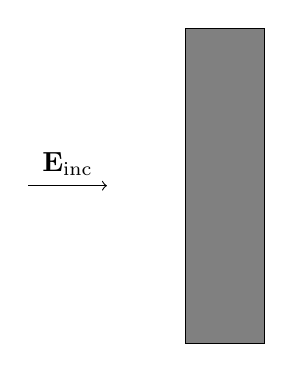
\begin{tikzpicture}
    \draw [fill=gray] (0, 2) rectangle (1, -2);
    \draw [->] (-2, 0) -- (-1, 0) node [pos =0.5, above] {$\mathbf{E}_\mathrm{inc}$};
  \end{tikzpicture}
\end{center}
A light wave is incident on the conductor, ie
\[
  \mathbf{E}_{\mathrm{inc}} = E_0 \hat{\mathbf{y}} \exp(i(kx + \omega t)),
\]
with $\omega = ck$.

We know that inside a conductor, $\mathbf{E} = 0$, and at the surface, $\mathbf{E}_{\parallel} = 0$. So $\mathbf{E}_0 \cdot \hat{\mathbf{y}}|_{x = 0} = 0$.

Then clearly our solution above does not satisfy the boundary conditions!

To achieve the boundary conditions, we add a reflected wave
\[
  \mathbf{E}_{\mathrm{ref}} = -E_0 \hat{\mathbf{y}} \exp(i(-kx - \omega t)).
\]
Then our total electric field is
\[
  \mathbf{E} = \mathbf{E}_{\mathrm{inc}} + \mathbf{E}_{\mathrm{ref}}.
\]
Then this is a solution to Maxwell's equations since it is a sum of two solutions, and satisfies $\mathbf{E}\cdot \hat{\mathbf{y}}|_{x = 0} = 0$ as required.

Maxwell's equations says $\nabla\times \mathbf{E} = -\frac{\partial \mathbf{B}}{\partial t}$. So
\begin{align*}
  \mathbf{B}_{\mathrm{inc}} &= \frac{E_0}{c}\hat{\mathbf{z}} \exp(i(kx - \omega t))\\
  \mathbf{B}_{\mathrm{ref}} &= \frac{E_0}{c}\hat{\mathbf{z}} \exp(i(-kx - \omega t))
\end{align*}
This obeys $\mathbf{B}\cdot \hat{\mathbf{n}} = 0$, where $\hat{\mathbf{n}}$ is the normal to the surface. But we also have
\[
  \mathbf{B}\cdot \hat{\mathbf{z}}|_{x = 0^-} = \frac{2E_0}{c}e^{-i\omega t},
\]
So there \emph{is} a magnetic field at the surface. However, we know that inside the conductor, we have $\mathbf{B} = 0$. This means that there is a discontinuity across the surface! We know that discontinuity happens when there is a surface current. Using the formula we've previously obtained, we know that the surface current is given by
\[
  \mathbf{K} = \pm\frac{2E_0}{\mu_0 c}\hat{\mathbf{y}} e^{-i \omega t}.
\]
So shining a light onto a metal will cause an oscillating current. We can imagine the process as the incident light hits the conductor, causes an oscillating current, which generates a reflected wave (since accelerating charges generate light --- cf.\ IID Electrodynamics)

We can do the same for light incident at an angle, and prove that the incident angle is equal to the reflected angle.

\subsection{Poynting vector}
Electromagnetic waves carry energy --- that's how the Sun heats up the Earth! We will compute how much.

The energy stored in a field in a volume $V$ is
\[
  U = \int_V \left(\frac{\varepsilon_0}{2}\mathbf{E}\cdot \mathbf{E} + \frac{1}{2\mu_0}\mathbf{B}\cdot \mathbf{B}\right)\;\d V.
\]
We have
\begin{align*}
  \frac{\d U}{\d t} &= \int_V \left(\varepsilon_0 \mathbf{E}\cdot \frac{\partial \mathbf{E}}{\partial t} + \frac{1}{\mu_0}\mathbf{B}\cdot \frac{\partial \mathbf{B}}{\partial t}\right)\;\d V\\
  &= \int_V \left(\frac{1}{\mu_0}\mathbf{E}\cdot (\nabla\times \mathbf{B}) - \mathbf{E}\cdot \mathbf{J} - \frac{1}{\mu_0}\mathbf{B}\cdot (\nabla\times \mathbf{E})\right)\;\d V.
\end{align*}
But
\[
  \mathbf{E}\cdot (\nabla \times \mathbf{B}) - \mathbf{B}\cdot (\nabla\times \mathbf{E}) = \nabla\cdot (\mathbf{E}\times \mathbf{B}),
\]
by vector identities. So
\[
  \frac{\d U}{\d t} = -\int_V \mathbf{J}\cdot \mathbf{E}\;\d V - \frac{1}{\mu_0}\int_S (\mathbf{E}\times \mathbf{B})\cdot \;\d \mathbf{S}.
\]
Recall that the work done on a particle $q$ moving with velocity $v$ is $\delta W = q\mathbf{v}\cdot \mathbf{E}\;\delta t$. So the $\mathbf{J}\cdot \mathbf{E}$ term is the work done on a charged particles in $V$. We can thus write
\begin{thm}[Poynting theorem]
  \[
    \underbrace{\frac{\d U}{\d t} + \int_V \mathbf{J}\cdot \mathbf{E} \;\d V}_{\text{Total change of energy in $V$ (fields + particles)}} = \underbrace{-\frac{1}{\mu_0}\int_S (\mathbf{E}\times \mathbf{B})\cdot\d S}_{\text{Energy that escapes through the surface }S}.
  \]
\end{thm}

\begin{defi}[Poynting vector]
  The \emph{Poynting vector} is
  \[
    \mathbf{S} = \frac{1}{\mu_0}\mathbf{E}\times \mathbf{B}.
  \]
\end{defi}
The Poynting vector characterizes the energy transfer.

For a linearly polarized wave,
\begin{align*}
  \mathbf{E} &= \mathbf{E}_0 \sin (\mathbf{k}\cdot \mathbf{x} - \omega t)\\
  \mathbf{B} &= \frac{1}{c}(\hat{\mathbf{k}}\times \mathbf{E}_0)\sin (\mathbf{k}\cdot \mathbf{x} - \omega t).
\end{align*}
So
\[
  \mathbf{S} = \frac{E_0^2}{c\mu_0}\hat{\mathbf{k}} \sin^2(\mathbf{k}\cdot\mathbf{x} - \omega t).
\]
The average over $T = \frac{2\pi}{\omega}$ is thus
\[
  \bra\mathbf{S}\ket = \frac{E_0^2}{2c\mu_0}\hat{\mathbf{k}}.
\]
\section{Electromagnetism and relativity}
In this section, we will write Maxwell's equations in the language of relativity, and show that the two are compatible. We will first start with a review of special relativity. We will introduce it in a more formal approach, forgetting about all that fun about time dilation, twins and spaceships.

\subsection{A review of special relativity}
\subsubsection{A geometric interlude on (co)vectors}
Let's first look at normal, Euclidean geometry we know from IA Vectors and Matrices. We all know what a vector is. A vector is, roughly, a direction. For example, the velocity of a particle is a vector --- it points in the direction where the particle is moving. On the other hand, position is not quite a vector. It is a vector only after we pick an ``origin'' of our space. Afterwards, we can think of position as a vector pointing the direction from the origin to where we are.

Perhaps a slightly less familiar notion is that of a \emph{covector}. A covector is some mathematical object that takes in a vector and spits out a number, and it has to do this in a linear way. In other words, given a vector space $V$, a covector is a linear map $V \to \R$.

One prominent example is that the derivative $\d f$ of a function $f: \R^n \to \R$ at (say) the origin is naturally a \emph{co}vector! If you give me a direction, the derivative tells us how fast $f$ changes in that direction. In other words, given a vector $\mathbf{v}$, $\d f(\mathbf{v})$ is the \emph{directional derivative} of $f$ in the direction of $\mathbf{v}$.

But, you say, we were taught that the derivative of $f$ is the gradient, which is a vector. Indeed, you've probably never heard of the word ``covector'' before. If we wanted to compute the directional derivative of $f$ in the direction of $v$, we simply compute the gradient $\nabla f$, and then take the dot product $\nabla f \cdot \mathbf{v}$. We don't need to talk about covectors, right?

The key realization is that to make the last statement, we need the notion of a dot product, or \emph{inner product}. Once we have an inner product, it is an easy mathematical fact that every covector $L: V \to \R$ is uniquely of the form
\[
  L(v) = \mathbf{v} \cdot \mathbf{w}
\]
for some fixed $\mathbf{w} \in V$, and conversely any vector gives a covector this way. Thus, whenever we have a dot product on our hands, the notion of covector is redundant --- we can just talk about vectors.

In special relativity, we still have an inner product. However, the inner product is not a ``genuine'' inner product. For example, the inner product of a (non-zero) vector with itself might be zero, or even negative! And in this case, we need to be careful about the distinction between a vector and a covector, and it is worth understanding the difference more carefully.

Since we eventually want to do computations, it is extremely useful to look at these in coordinates. Suppose we have picked a basis $\mathbf{e}_1, \cdots, \mathbf{e}_n$. Then by definition of a basis, we can write any vector $\mathbf{v}$ as $\mathbf{v} = \sum v^i \mathbf{e}_i$. These $v^i$ are the coordinates of $\mathbf{v}$ in this coordinate system, and by convention, we write the indices with superscript. We also say they have \emph{upper indices}.

We can also introduce coordinates for \emph{co}vectors. If $L$ is a covector, then we can define its coordinates by
\[
  L_i = L(\mathbf{e}_i).
\]
By convention, the indices are now written as subscripts, or \emph{lower indices}. Using the summation convention, we have
\[
  L(\mathbf{v}) = L(v^i \mathbf{e}_i) = v^i L(\mathbf{e}_i) = v^i L_i.
\]
Previously, when we introduced the summation convention, we had a ``rule'' that each index can only appear at most twice, and we sum over it when it is repeated. Here we can refine this rule, and give good meaning to it:
\begin{rrule}
  We can only contract an upper index with a lower index.
\end{rrule}
The interpretation is that ``contraction'' really just means applying a covector to a vector --- a very natural thing to do. It doesn't make sense to ``apply'' a vector to a vector, or a covector to a covector. It also doesn't make sense to repeat the same index three times, because we can only apply a single covector to a single vector.

It is common to encounter some things that are neither vectors nor covectors, but we still want to apply the summation convention to them. For example, we want to write $\mathbf{v} = v^i \mathbf{e}_i$, even though $\mathbf{e}_i$ is not a covector. It turns out in all cases we encounter, there is one choice of upper or lower indexing that makes it consistent with our summation convention. For example, we should write $\mathbf{e}_i$, not $\mathbf{e}^i$, so that $\mathbf{v} = v^i \mathbf{e}_i$ works out.

We said previously that the existence of an inner product allows us to convert a covector into a vector, and vice versa. So let's see how inner products work in a choice of basis.

If the basis we picked were orthonormal, then for any vectors $\mathbf{v}$ and $\mathbf{w}$, we simply have $\mathbf{v} \cdot \mathbf{w} = \mathbf{v}^T \mathbf{w}$. Alternatively, we have $\mathbf{v} \cdot \mathbf{w} = \sum_i v^i w^i$. If our basis were not orthonormal (which is necessarily the case in SR), we can define the matrix $\boldsymbol\eta$ by
\[
  \eta_{ij} = \mathbf{e}_i \cdot \mathbf{e}_j.
\]
We will later say that $\boldsymbol\eta$ is a $(0, 2)$-tensor, after we defined what that means. The idea is that it takes in \emph{two} vectors, and returns a number (namely the inner product of them). This justifies our choice to use lower indices for both coordinates. For now, we can argue for this choice by noting that the indices on $\mathbf{e}_i$ and $\mathbf{e}_j$ are already lower.

Using this $\boldsymbol\eta$, we can compute
\[
  \mathbf{v} \cdot \mathbf{w} = (v^i \mathbf{e}_i) \cdot (w^j \mathbf{e}_j) = v^i w^j (\mathbf{e}_i \cdot \mathbf{e}_j) = w^i w^j \eta_{ij}.
\]
In other words, we have
\[
  \mathbf{v} \cdot \mathbf{w} = \mathbf{v}^T \boldsymbol\eta \mathbf{w}.
\]
We see that this matrix $\boldsymbol\eta$ encodes all the information about the inner product in this basis. This is known as the \emph{metric}. If we picked an orthonormal basis, then $\boldsymbol\eta$ would be the identity matrix.

Now it is easy to convert a vector into a covector. The covector $(-\cdot \mathbf{w})$ is given by $\mathbf{v} \cdot \mathbf{w} = v^i (w^j\eta_{ij})$. We can then read off the coordinates of the covector to be
\[
  w_i = w^j \eta_{ij}.
\]
In general, these coordinates $w_i$ are \emph{not} the same as $w^i$. This is generally true only if $\eta_{ij}$ is the identity matrix, i,e.\ the basis is orthonormal. Thus, distinguishing between vectors and covectors now has a practical purpose. Each ``vector'' has two sets of coordinates --- one when you think of it as a vector, and one when you turn it into a covector, and they are different. So the positioning of the indices help us keep track of which coordinates we are talking about.

We can also turn a covector $w_i$ back to a vector, if we take the inverse of the matrix $\boldsymbol\eta$, which we will write as $\eta^{ij}$. Then
\[
  w^i = w_j \eta^{ij}.
\]
\subsubsection{Transformation rules}
It is often the case that in relativity, we can write down the coordinates of an object in any suitable basis. However, it need not be immediately clear to us whether that object should be a vector or covector, or perhaps neither. Thus, we need a way to identify whether objects are vectors or covectors. To do so, we investigate how the coordinates of vectors and covectors when we change basis.

By definition, if we have a change of basis matrix $P$, then the coordinates of a vector transform as $\mathbf{v} \mapsto P \mathbf{v}$, or equivalently
\[
  v^i \mapsto v'^i = P^i\!_j v^j.
\]
How about covectors? If $L$ is a covector and $\mathbf{v}$ is vector, then $L(\mathbf{v})$ is a number. In particular, its value does not depend on basis. Thus, we know that the sum $L_i v^i$ must be invariant under any change of basis. Thus, if $L_i \mapsto \tilde{L}_i$, then we know
\[
  \tilde{L}_i P^i\!_j v^j = L_i v^j.
\]
Thus, we know $\tilde{L}_i P^i\!_j = L_i$. To obtain $\tilde{L}_i$, we have to invert $P^i\!_j$ and multiply $L_i$ with that.

However, our formalism in terms of indices does not provide us with a way of denoting the inverse of a matrix pleasantly. We can avert this problem by focusing on \emph{orthogonal} matrices, i.e.\ the matrices that preserve the metric. We say $P$ is orthogonal if
\[
  P^T \eta P = \eta,
\]
or equivalently,
\[
  P^i\!_j \eta_{ik} P^k\!_\ell = \eta_{j\ell}.
\]
This implies the inverse of $P$ has coordinates
\[
  P_i{}^j = (\eta^{-1} P^T \eta)_i\!^j = \eta_{i\ell} \eta^{jk} P^\ell\!_k,
\]
which is the fancy way of describing the ``transpose'' (which is not the literal transpose unless $\eta = I$). This is just reiterating the fact that the inverse of an orthogonal matrix is its transpose. When we do special relativity, the orthogonal matrices are exactly the Lorentz transformations.

Thus, we find that if $P$ is orthogonal, then covectors transform as
\[
  L_i \mapsto L_i' = P_i{}^j L_j.
\]
We can now write down the ``physicists' '' definition of vectors and covectors. Before we do that, we restrict to the case of interest in special relativity. The reason is that we started off this section with the caveat ``in any \emph{suitable} basis''. We shall not bother to explain what ``suitable'' means in general, but just do it in the case of interest.

\subsubsection{Vectors and covectors in SR}
Recall from IA Dynamics and Relativity that in special relativity, we combine space and time into one single object. For example, the position and time of an event is now packed into a single \emph{4-vector} in spacetime
\[
  X^\mu =
  \begin{pmatrix}
    ct\\
    x\\
    y\\
    z
  \end{pmatrix}.
\]
Here the index $\mu$ ranges from $0$ to $3$. In special relativity, we use Greek alphabets (e.g.\ $\mu, \nu, \rho, \sigma$) to denote the indices. If we want to refer to the spacial components ($1, 2, 3$) only, we will use Roman alphabets (e.g.\ $i, j, k$) to denote them.

As we initially discussed, position is very naturally thought of as a vector, and we will take this as our starting postulate. We will then use the transformation rules to identify whether any other thing should be a vector or a covector.

In the ``standard'' basis, the metric we use is the \term{Minkowski metric}, defined by
\[
  \eta_{\mu\nu} =
  \begin{pmatrix}
    +1 & 0 & 0 & 0\\
    0 & -1 & 0 & 0\\
    0 & 0 & -1 & 0\\
    0 & 0 & 0 & -1
  \end{pmatrix}.\tag{$*$}
\]
This is \emph{not} positive definite, hence not a genuine inner product. However, it is still invertible, which is what our previous discussion required. This means, for example,
\[
  X \cdot X = (ct)^2 - (x^2 + y^2 + z^2),
\]
the spacetime interval.

\begin{defi}[Orthonormal basis]
  An \emph{orthonormal basis} of spacetime is a basis where the metric takes the form $(*)$. An (orthonormal) coordinate system is a choice of orthonormal basis.
\end{defi}

\begin{defi}[Lorentz transformations]
  A \emph{Lorentz transformation} is a change-of-basis matrix that preserves the inner product, i.e.\ orthogonal matrices under the Minkowski metric.
\end{defi}
Thus, Lorentz transformations send orthonormal bases to orthonormal bases. For example, the familiar Lorentz boost
\begin{align*}
  ct' &= \gamma\left(ct - \frac{v}{c}x\right)\\
  x' &= \gamma\left(x - \frac{v}{c}ct\right)\\
  y' &= y\\
  z' &= z
\end{align*}
is the Lorentz transformation given by the matrix
\[
  \Lambda^\mu\!_\nu =
  \begin{pmatrix}
    \gamma & -\gamma v/c & 0 &0\\
    -\gamma v/c & \gamma & 0 & 0\\
    0 & 0 & 1 & 0\\
    0 & 0 & 0 & 1
  \end{pmatrix}
\]
Other examples include rotations of the space dimensions, which are given by matrices of the form
\[
  \Lambda^\mu\!_\nu =
  \begin{pmatrix}
    1 & 0 & 0 & 0\\
    0 & \\
    0 & & R \\
    0
  \end{pmatrix},
\]
with $R$ a rotation matrix.

We can now write down our practical definition of vectors and covectors.
\begin{defi}[Vectors and covectors]
  A vector is an assignment of $4$ numbers $V^\mu, \mu = 0, 1, 2, 3$ to each coordinate system such that under a change of basis by $\Lambda$, the coordinates $V^\mu$ transform as $V^\mu \mapsto \Lambda^\mu\!_\nu V^\nu$.

  A covector is an assignment of $4$ numbers $V_\mu, \mu = 0, 1, 2, 3$ to each coordinate system such that under a change of basis by $\Lambda$, the coordinates $V_\mu$ transform as $V_\mu \mapsto \Lambda_\mu\!^\nu V_\nu$.
\end{defi}

\begin{eg}
  By assumption, the position $X^\mu$ is a vector.
\end{eg}

\begin{eg}
  Suppose we have a trajectory of a particle $X^\mu(s)$ in spacetime. Then $\frac{\d}{\d s} X^\mu(s)$ is also a vector, by checking it transforms.
\end{eg}

Finally, we would want to be able to talk about tensors. For example, we want to be able to talk about $X^\mu X^\nu$. This is an assignment of $16$ numbers indexed by $\mu, \nu = 0, 1, 2, 3$ that transforms as
\[
  X^\mu X^\nu \mapsto \Lambda^\mu\!_\rho \Lambda^\nu\!_\sigma X^\rho X^\sigma.
\]
We would also like to talk about $\eta_{\mu\nu}$ as a tensor. We can make the following general definition:

\begin{defi}[Tensor]
  A \emph{tensor} of type $(m, n)$ is a quantity
  \[
    T^{\mu_1\cdots \mu_n}\!_{\nu_1\cdots \nu_n}
  \]
  which transforms as
  \[
    T'^{\mu_1\cdots \mu_n}\!_{\nu_1\cdots \nu_n} = \Lambda^{\mu_1}\!_{\rho_1} \cdots \Lambda^{\mu_m}\!_{\rho_m}\Lambda_{\nu_1}\!^{\sigma_1}\cdots\Lambda_{\nu_n}\!^{\sigma_n} \times T^{\rho_1, \cdots, \rho_m}\!_{\sigma_1, \cdots, \sigma_n}.
  \]
\end{defi}
As we saw, we can change the type of a tensor by raising and lowering indices by contracting with $\eta_{\mu\nu}$ or its inverse. However, the total $n + m$ will not be changed.

Finally, we introduce the $4$-derivative.
\begin{defi}[4-derivative]
  The \emph{4-derivative} is
  \[
    \partial_\mu = \frac{\partial}{\partial X^\mu} = \left(\frac{1}{c}\frac{\partial}{\partial t}, \nabla\right).
  \]
\end{defi}
As we previously discussed, the derivative ought to be a covector. We can also verify this by explicit computation using the chain rule. Under a transformation $X^\mu \mapsto X'^\mu$, we have
\begin{align*}
  \partial_\mu = \frac{\partial}{\partial X^\mu} \mapsto \frac{\partial}{\partial X'^\mu} = \frac{\partial X^\nu}{\partial X'^\mu}\frac{\partial}{\partial X^\nu} = (\Lambda^{-1})^\nu\!_\mu\partial_\nu = \Lambda_\mu\!^\nu \partial_\nu.
\end{align*}

\subsection{Conserved currents}
Recall the continuity equation
\[
  \frac{\partial\rho}{\partial t} + \nabla\cdot \mathbf{J} = 0.
\]
An implication of this was that we cannot have a charge disappear on Earth and appear on Moon. One way to explain this impossibility would be that the charge is travelling faster than the speed of light, which is something related to relativity. This suggests that we might be able to write it relativistically.

We define
\[
  J^\mu =
  \begin{pmatrix}
    \rho c\\
    \mathbf{J}
  \end{pmatrix}
\]
Before we do anything with it, we must show that this is a 4-vector, i.e.\ it transforms via left multiplication by $\Lambda^\mu\!_\nu$.

The full verification is left as an exercise. We work out a special case to justify why this is a sensible thing to believe in. Suppose we have a static charge density $\rho_0(\mathbf{x})$ with $\mathbf{J} = 0$. In a frame boosted by $\mathbf{v}$, we want to show that the new current is
\[
  J'^\mu = \Lambda^\mu\!_\nu J^\nu =
  \begin{pmatrix}
    \gamma \rho_0 c\\
    -\gamma \rho_0 \mathbf{v}
  \end{pmatrix}.
\]
The new charge is now $\gamma \rho_0$ instead of $\rho_0$. This is correct since we have Lorentz contraction. As space is contracted, we get more charge per unit volume. Then the new current is velocity times charge density, which is $\mathbf{J}' = \gamma\rho_0 \mathbf{v}$.

With this definition of $J^\mu$, local charge conservation is just
\[
  \partial_\mu J^\mu = 0.
\]
This is invariant under Lorentz transformation, simply because the indices work out (i.e.\ we match indices up with indices down all the time).

We see that once we have the right notation, the laws of physics are so short and simple!

\subsection{Gauge potentials and electromagnetic fields}
Recall that when solving electrostatic and magentostatic problems, we introduced the potentials $\varphi$ and $\mathbf{A}$ to help solve two of Maxwell's equations:
\begin{align*}
  \nabla\times \mathbf{E} = 0 &\Leftrightarrow \mathbf{E} = -\nabla \phi\\
  \nabla\cdot \mathbf{B} = 0 &\Leftrightarrow \mathbf{B} = \nabla\times \mathbf{A}.
\end{align*}
However, in general, we do not have $\nabla \times \mathbf{E} = 0$. Instead, the equations are
\[
  \nabla\times E + \frac{\partial \mathbf{B}}{\partial t} = 0,\quad \nabla\cdot \mathbf{B} = 0.
\]
So we cannot use $\mathbf{E} = -\nabla \phi$ directly if $\mathbf{B}$ changes. Instead, we define $\mathbf{E}$ and $\mathbf{B}$ in terms of $\phi$ and $\mathbf{A}$ as follows:
\begin{align*}
  \mathbf{E} &= -\nabla\phi - \frac{\partial \mathbf{A}}{\partial t}\\
  \mathbf{B} &= \nabla\times \mathbf{A}.
\end{align*}
It is important to note that $\phi$ and $\mathbf{A}$ are not unique. We can shift them by
\begin{align*}
  \mathbf{A} \mapsto \mathbf{A} + \nabla \chi\\
  \phi \mapsto \phi - \frac{\partial \chi}{\partial t}
\end{align*}
for any function $\chi(\mathbf{x}, t)$. These are known as \emph{gauge transformations}. Plug them into the equations and you will see that you get the same $\mathbf{E}$ and $\mathbf{B}$.

Now we have ended up with four objects, 1 from $\phi$ and 3 from $\mathbf{A}$, so we can put them into a 4-vector \emph{gauge potential}:
\[
  A^\mu =
  \begin{pmatrix}
    \phi/c\\
    \mathbf{A}
  \end{pmatrix}\]
We will assume that this makes sense, i.e.\ is a genuine 4-vector.

Now gauge transformations take a really nice form:
\[
  A_\mu \mapsto A_\mu - \partial_\mu\chi.
\]
Finally, we define the anti-symmetric electromagnetic tensor
\[
  F_{\mu\nu} = \partial_\mu A_\nu -\partial_\nu A_\mu.
\]
Since this is antisymmetric, the diagonals are all 0, and $A_{\mu\nu} = -A_{\nu\mu}$. So this thing has $(4 \times 4 - 4)/2 = 6$ independent components. So it could encapsulate information about the electric and magnetic fields (and nothing else).

We note that $F$ is invariant under gauge transformations:
\[
  F_{\mu\nu} \mapsto F_{\mu\nu} - \partial_\mu\partial_\nu\chi + \partial_\nu\partial_\mu \chi = F_{\mu\nu}.
\]
We can compute components of $F_{\mu\nu}$.
\[
  F_{01} = \frac{1}{c}\frac{\partial}{\partial t}(-A_x) - \frac{\partial \phi/c}{\partial x} = \frac{E_x}{c}.
\]
Note that we have $-A_x$ instead of $A_x$ since $F_{\mu\nu}$ was defined in terms of $A_\mu$ with indices down. We can similarly obtain $F_{02} = E_y/c$ and $F_{03} = E_z/c$.

We also have
\[
  F_{12} = \frac{\partial}{\partial x}(-Ay) - \frac{\partial}{\partial y}(-A_x) = -B_z.
\]
So
\[
  F_{\mu\nu} =
  \begin{pmatrix}
    0 & E_x/c & E_y/c & E_z/c\\
    -E_x/c & 0 & -B_z & B_y\\
    -E_y/c & B_z & 0 & -B_x\\
    -E_z/c & -B_y & B_x & 0
  \end{pmatrix}
\]
Raising both indices, we have
\[
  F^{\mu\nu} = \eta^{\mu\rho}\eta^{\nu\sigma} F_{\rho\sigma} =
  \begin{pmatrix}
    0 & -E_x/c & -E_y/c & -E_z/c\\
    E_x/c & 0 & -B_z & B_y\\
    E_y/c & B_z & 0 & -B_x\\
    E_z/c & -B_y & B_x & 0
  \end{pmatrix}
\]
So the electric fields are inverted and the magnetic field is intact (which makes sense, since moving indices up and down will flip the sign of the spacial components. The electric field has one, while the magnetic field has two. So the magnetic field is swapped twice and is intact).

Both $F_{\mu\nu}$ and $F^{\mu\nu}$ are tensors. Under a Lorentz transformation, we have
\[
  F'^{\mu\nu} = \Lambda^\mu\!_\rho\Lambda^\nu_\sigma F^{\rho\sigma}.
\]
For example under rotation
\[
  \Lambda =
  \begin{pmatrix}
    1 & 0 & 0 & 0\\
    0\\
    0 & & R\\
    0
  \end{pmatrix},
\]
we find that
\begin{align*}
  \mathbf{E}' &= R\mathbf{E}\\
  \mathbf{B}' &= R\mathbf{B}.
\end{align*}
Under a boost by $v$ in the $x$-direction , we have
\begin{align*}
  E_x' &= E_x\\
  E_y' &= \gamma(E_y - vB_z)\\
  E_z' &= \gamma(E_z + vB_y)\\
  B_x' &= B_x\\
  B_y' &= \gamma\left(B_y + \frac{v}{c^2}E_z\right)\\
  B_z' &= \gamma\left(B_z - \frac{v}{c^2} E_y\right)
\end{align*}

\begin{eg}[Boosted line charge]
  An infinite line along the $x$ direction with uniform charge per unit length, $\eta$, has electric field
  \[
    \mathbf{E} = \frac{\eta}{2\pi \varepsilon_0 (y^2 + z^2)}
    \begin{pmatrix}
      0\\ y\\ z
    \end{pmatrix}.
  \]
  The magnetic field is $\mathbf{B} = 0$. Plugging this into the equation above, an observer in frame $S'$ boosted with $\mathbf{v} = (v, 0, 0)$, i.e.\ parallel to the wire, sees
  \[
    \mathbf{E} = \frac{\eta\gamma}{2\pi\varepsilon_0(y^2 + z^2)}
    \begin{pmatrix}
      0\\y\\z
    \end{pmatrix} =
    \frac{\eta\gamma}{2\pi\varepsilon_0(y'^2 + z'^2)}
    \begin{pmatrix}
      0\\y'\\z'
    \end{pmatrix}.
  \]
  Also,
  \[
    \mathbf{B} = \frac{\eta\gamma v}{2\pi\varepsilon_0 \sigma^2(y^2 + z^2)}
    \begin{pmatrix}
      0\\z\\-y
    \end{pmatrix} = \frac{\eta\gamma v}{2\pi\varepsilon_0 \sigma^2(y'^2 + z'^2)}
    \begin{pmatrix}
      0\\z'\\-y'
    \end{pmatrix}.
  \]
  In frame $S'$, the charge density is Lorentz contracted to $\gamma\eta$. The magnetic field can be written as
  \[
    \mathbf{B} = \frac{\mu_0 I'}{2\pi \sqrt{y'^2 + z'^2}}\, \hat{\varphi}',
  \]
  where $\displaystyle \hat{\varphi}' = \frac{1}{\sqrt{y'^2 + z'^2}} \begin{pmatrix}0\\-z'\\y'\end{pmatrix}$ is the basis vector of cylindrical coordinates, and $I' = -\gamma\eta v$ is the current.

  This is what we calculated from Ampere's law previously. But we didn't \emph{use} Ampere's law here. We used Gauss' law, and then applied a Lorentz boost.
\end{eg}
We see that magnetic fields are relativistic effects of electric fields. They are what we get when we apply a Lorentz boost to an electric field. So relativity is not only about \emph{very fast objects}\textsuperscript{TM}. It is there when you stick a magnet onto your fridge!

\begin{eg}[Boosted point charge]
  A boosted point charge generates a current, but is not the steady current we studied in magnetostatics. As the point charge moves, the current density moves.

  A point charge $Q$, at rest in frame $S$ has
  \[
    \mathbf{E} = \frac{Q}{4\pi \varepsilon_0 r^2}\hat{\mathbf{r}} = \frac{Q}{4\pi \varepsilon_0^2(x^2 + y^2 + z^2)^{3/2}}
    \begin{pmatrix}
      x\\y\\z
    \end{pmatrix},
  \]
  and $\mathbf{B} = 0$.

  In frame $S'$, boosted with $\mathbf{v} = (v, 0, 0)$, we have
  \[
    \mathbf{E}' = \frac{Q}{4\pi \varepsilon_0(x^2 + y^2 + z^2)^{3/2}}
    \begin{pmatrix}
      x\\ \gamma y\\ \gamma z.
    \end{pmatrix}.
  \]
  We need to express this in terms of $x', y', z'$, instead of $x, y, z$. Then we get
  \[
    \mathbf{E}' = \frac{Q\gamma}{4\pi \varepsilon_0 (\gamma^2(x' + vt')^2 + y'^2 + z'^2)^{3/2}}
    \begin{pmatrix}
      x' + vt'\\y'\\z'
    \end{pmatrix}.
  \]
  Suppose that the particle sits at $(-vt', 0, 0)$ in $S'$. Let's look at the electric at $t'=0$. Then the radial vector is $\mathbf{r}' =
  \begin{pmatrix}
    x'\\y'\\z'
  \end{pmatrix}.
  $
  In the denominator, we write
  \begin{align*}
    \gamma^2x'^2 + y'^2 + z'^2 &= (\gamma^2 - 1)x'^2 + r'^2\\
    &= \frac{v^2\gamma^2}{c^2}x'^2 + r'^2\\
    &= \left(\frac{v^2\gamma^2}c^2 \cos^2 \theta + 1\right)r'^2\\
    &= \gamma^2\left(1 - \frac{v^2}{c^2}\sin^2 \theta\right)r'^2
  \end{align*}
  where $\theta$ is the angle between the $x'$ axis and $\mathbf{r}'$.

  So
  \[
    \mathbf{E}' = \frac{1}{\gamma^2\left(1 - \frac{v^2}{c^2}\sin^2 \theta\right)^{3/2}}\frac{Q}{4\pi \varepsilon_0 r^2}\hat{\mathbf{r}'}.
  \]
  The factor $1/\gamma^2\left(1 - \frac{v^2}{c^2}\sin^2 \theta\right)^{3/2}$ squashes the electric field in the direction of motion.

  This result was first discovered by Lorentz from solving Maxwell's equations directly, which lead to him discovering the Lorentz transformations.

  There is also a magnetic field
  \[
    \mathbf{B} = \frac{\mu_0 Q\gamma v}{4\pi(\gamma^2(x' + vt')^2 + y'^2 + z'^2)^{3/2}}
    \begin{pmatrix}
      0\\z'\\-y'
    \end{pmatrix}.
  \]
\end{eg}

\subsubsection*{Lorentz invariants}
We can ask the question ``are there any combinations of $\mathbf{E}$ and $\mathbf{B}$ that all observers agree on?'' With index notation, all we have to do is to contract all indices such that there are no dangling indices.

It turns out that there are two such possible combinations.

The first thing we might try would be
\[
  \frac{1}{2}F_{\mu\nu}F^{\mu\nu} = -\frac{\mathbf{E}^2}{c^2} + \mathbf{B}^2,
\]
which works great.

To describe the second invariant, we need to introduce a new object in Minkowski space. This is the fully anti-symmetric tensor
\[
  \varepsilon^{\mu\nu\rho\sigma} =
  \begin{cases}
    +1 & \mu\nu\rho\sigma\text{ is even permutation of 0123}\\
    -1 & \mu\nu\rho\sigma\text{ is odd permutation of 0123}\\
    0 & \text{otherwise}
  \end{cases}
\]
This is analogous to the $\varepsilon_{ijk}$ in $\R^3$, just that this time we are in 4-dimensional spacetime. Under a Lorentz transformation,
\[
  \varepsilon'^{\mu\nu\rho\sigma} = \Lambda^\mu\!_\kappa\Lambda^\nu\!_\lambda \Lambda^\rho\!_\alpha \Lambda^\sigma\!_\beta \varepsilon^{\kappa\lambda\alpha\beta}.
\]
Since $\varepsilon^{\mu\nu\rho\sigma}$ is fully anti-symmetric, so is $\varepsilon'^{\mu\nu\rho\sigma}$. Similar to what we did in $\R^3$, we can show that the only fully anti-symmetric tensors in Minkowski space are multiples of $\varepsilon^{\mu\nu\rho\sigma}$. So
\[
  \varepsilon'^{\mu\nu\rho\sigma} = a \varepsilon^{\mu\nu\rho\sigma}
\]
for some constant $a$. To figure out what $a$ is, test a single component:
\[
  \varepsilon'^{0123} = \Lambda^0\!_\kappa\Lambda^1\!_\lambda \Lambda^2\!_\beta \Lambda^3\!_\beta \varepsilon^{\kappa\lambda\alpha\beta} = \det \Lambda.
\]
Lorentz transformations have $\det \Lambda = +1$ (rotations, boosts), or $\det \Lambda = -1$ (reflections, time reversal).

We will restrict to $\Lambda$ such that $\det \Lambda = +1$. Then $a = 1$, and $\varepsilon^{\mu\nu\rho\sigma}$ is invariant. In particular, it is a tensor.

We can finally apply this to electromagnetic fields. The \emph{dual electromagnetic tensor} is defined to be
\[
  \tilde{F}^{\mu\nu} = \frac{1}{2}\varepsilon^{\mu\nu\rho\sigma}F_{\rho\sigma}.=
  \begin{pmatrix}
    0 & -B_x & -B_y & -B_z\\
    B_x & 0 & E_z/c & -E_y/c\\
    B_y & -E_z/c & 0 & E_x/c\\
    B_z & E_y/c & -E_x/c & 0
  \end{pmatrix}.
\]
Why do we have the factor of a half? Consider a single component, say $\tilde{F}^{12}$. It gets contributions from both $F_{03}$ and $F_{30}$, so we need to average the sum to avoid double-counting. $\tilde{F}^{\mu\nu}$ is yet another antisymmetric matrix.

This is obtained from $F^{\mu\nu}$ through the substitution $\mathbf{E} \mapsto c\mathbf{B}$ and $\mathbf{B}\mapsto -\mathbf{E}/c$. Note the minus sign!

Then $\tilde{F}^{\mu\nu}$ is a tensor. We can construct the other Lorentz invariant using $\tilde{F}^{\mu\nu}$. We don't get anything new if we contract this with itself, since $\tilde{F}_{\mu\nu}\tilde{F}^{\mu\nu} = -F_{\mu\nu}F^{\mu\nu}$. Instead, the second Lorentz invariant is
\[
  \frac{1}{4}\tilde{F}^{\mu\nu}F_{\mu\nu} = \mathbf{E}\cdot \mathbf{B}/c.
\]
\subsection{Maxwell Equations}
To write out Maxwell's Equations relativistically, we have to write them out in the language of tensors. It turns out that they are
\begin{align*}
  \partial_\mu F^{\mu\nu} &= \mu_0 J^\nu\\
  \partial_\mu \tilde{F}^{\mu\nu} &= 0.
\end{align*}
As we said before, if we find the right way of writing equations, they look really simple! We don't have to worry ourselves with where the $c$ and $\mu_0$, $\varepsilon_0$ go!

Note that each law is actually 4 equations, one for each of $\nu = 0, 1, 2, 3$. Under a Lorentz boost, the equations are not invariant individually. Instead, they all transform nicely by left-multiplication of $\Lambda_\rho^\nu$.

We now check that these agree with the Maxwell's equations.

First work with the first equation: when $\nu = 0$, we are left with
\[
  \partial_i F^{i0} = \mu_0 J^0,
\]
where $i$ ranges over $1, 2, 3$. This is equivalent to saying
\[
  \nabla\cdot \left(\frac{\mathbf{E}}{c}\right) = \mu_0 \rho c,
\]
or
\[
  \nabla\cdot \mathbf{E} = c^2 \mu_0 \rho = \frac{\rho}{\varepsilon_0}
\]
When $\nu = i$ for some $i = 1, 2, 3$, we get
\[
  \partial _\mu F^{\mu i} = \mu_0 J^i.
\]
So after some tedious calculation, we obtain
\[
  \frac{1}{c}\frac{\partial}{\partial t}\left(-\frac{\mathbf{E}}{c}\right) + \nabla\times \mathbf{B} = \mu_0 \mathbf{J}.
\]
With the second equation, when $\nu = 0$, we have
\[
  \partial_i \tilde{F}^{i0} = 0 \Rightarrow \nabla\cdot \mathbf{B} = 0.
\]
$\nu = i$ gives
\[
  \partial_\mu \tilde{F}^{\mu i} = 0 \Rightarrow \frac{\partial \mathbf{B}}{\partial t} + \nabla\times \mathbf{E}.
\]
So we recover Maxwell's equations. Then we now see why the $J^\nu$ term appears in the first equation and not the second --- it tells us that there is only electric charge, not magnetic charge.

We can derive the continuity equation from Maxwell's equation here. Since $\partial_\nu\partial_\mu F^{\mu\nu} = 0$ due to anti-symmetry, we must have $\partial_\nu J^\nu = 0$. Recall that we once derived the continuity equation from Maxwell's equations without using relativity, which worked but is not as clean as this.

Finally, we recall the long-forgotten potential $A_\mu$. If we define $F_{\mu\nu}$ in terms of it:
\[
  F_{\mu\nu} = \partial_\mu A_\nu - \partial_\nu A_\mu,
\]
then the equation $\partial_\mu \tilde{F}^{\mu\nu} = 0$ comes for free since we have
\[
  \partial_\mu \tilde{F}^{\mu\nu} = \frac{1}{2}\varepsilon^{\mu\nu\rho\sigma}\partial_{\mu}F_{\rho\sigma} = \frac{1}{2} \varepsilon^{\mu\nu\rho\sigma}\partial_\mu(\partial_\rho A_\sigma - \partial_\sigma A_\rho) = 0
\]
by symmetry. This means that we can also write the Maxwell equations as
\[
  \partial_\mu F^{\mu\nu} = \mu_0 J^\nu\quad\text{where}\quad F_{\mu\nu} = \partial_\mu A_\nu - \partial_\nu A_\mu.
\]
\subsection{The Lorentz force law}
The final aspect of electromagnetism is the Lorentz force law for a particle with charge $q$ moving with velocity $\mathbf{u}$:
\[
  \frac{\d \mathbf{p}}{\d t} = q(\mathbf{E} + \mathbf{v}\times \mathbf{B}).
\]
To write this in relativistic form, we use the proper time $\tau$ (time experienced by particle), which obeys
\[
  \frac{\d t}{\d \tau} = \gamma(\mathbf{u}) = \frac{1}{\sqrt{1 - u^2/c^2}}.
\]
We define the 4-velocity $\displaystyle U = \frac{\d X}{\d \tau} = \gamma\begin{pmatrix}c\\ \mathbf{u}\end{pmatrix}$, and 4-momentum $P = \begin{pmatrix}E/c\\ \mathbf{p}\end{pmatrix}$, where $E$ is the energy. Note that $E$ is the energy while $\mathbf{E}$ is the electric field.

The Lorentz force law can be written as
\[
  \frac{\d P^\mu}{\d \tau} = qF^{\mu\nu}U_\nu.
\]
We show that this does give our original Lorentz force law:

When $\mu = 1, 2, 3$, we obtain
\[
  \frac{\d \mathbf{p}}{\d \tau} = q\gamma (\mathbf{E} + \mathbf{v}\times \mathbf{B}).
\]
By the chain rule, since $\frac{\d t}{\d \tau} = \gamma$, we have
\[
  \frac{\d \mathbf{p}}{\d t} = q(\mathbf{E}+ \mathbf{v}\times \mathbf{B}).
\]
So the good, old Lorentz force law returns. Note that here $\mathbf{p} = m\gamma \mathbf{v}$, the relativistic momentum, not the ordinary momentum.

But how about the $\mu = 0$ component? We get
\[
  \frac{\d P^0}{\d \tau} = \frac{1}{c}\frac{\d E}{\d \tau} = \frac{q}{c}\gamma \mathbf{E}\cdot \mathbf{v}.
\]
This says that
\[
  \frac{\d E}{\d t} = q\mathbf{E}\cdot \mathbf{v},
\]
which is our good old formula for the work done by an electric field.

\begin{eg}[Motion in a constant field]
  Suppose that $\mathbf{E} = (E, 0, 0)$ and $\mathbf{u} = (v, 0, 0)$. Then
  \[
    m\frac{\d (\gamma u)}{\d t} = qE.
  \]
  So
  \[
    m\gamma u = qEt.
  \]
  So
  \[
    u = \frac{\d x}{\d t} = \frac{qEt}{\sqrt{m^2 + q^2 E^2 t^2/c^2}}.
  \]
  Note that $u\to c$ as $t\to \infty$. Then we can solve to find
  \[
    x = \frac{mc^2}{q}\left(\sqrt{1 + \frac{q^2 E^2 t^2}{mc^2}} - 1\right)
  \]
  For small $t$, $x\approx \frac{1}{2}qEt^2$, as expected.
\end{eg}

\begin{eg}[Motion in constant magnetic field]
  Suppose $\mathbf{B} = (0, 0, B)$. Then we start with
  \[
    \frac{\d P^0}{\d \tau} = 0 \Rightarrow E = m\gamma c^2 = \text{constant}.
  \]
  So $|\mathbf{u}|$ is constant. Then
  \[
    m\frac{\partial (\gamma \mathbf{u})}{\partial t} = q\mathbf{u}\times \mathbf{B}.
  \]
  So
  \[
    m\gamma \frac{\d \mathbf{u}}{\d t} = q\mathbf{u}\times \mathbf{B}
  \]
  since $|\mathbf{u}|$, and hence $\gamma$, is constant. This is the same equation we saw in Dynamics and Relativity for a particle in a magnetic field, except for the extra $\gamma$ term. The particle goes in circles with frequency
  \[
    \omega = \frac{qB}{m\gamma}.
  \]
\end{eg}
\end{document}
